\documentclass[11pt]{report}
\usepackage[utf8]{inputenc}
\usepackage[margin=1.0in]{geometry}
\usepackage[titlepage]{lib/makesubtitle}

\title{CIS 3715 Final Project Report}
\subtitle{Using satellite imagery to train a model for identifying the type of landmarks.}
\author{Leomar Durán}
\date{April 2022}

% for the Jupyter notebook
\usepackage{lib/ipynb}
\usepackage{minted}

% line spacing, paragraph indentation
\usepackage{setspace}
\singlespacing
\setlength\parindent{0.25in}

% hyperlinks
\usepackage{hyperref}

% remove level 1 margin on any list
\usepackage[inline]{enumitem}
\setlist[1]{leftmargin=0in}

% non-floating figures and tables
\usepackage{lib/nonfloatenvirons}
% table width, rules, row spacing
\usepackage{tabularx}
\usepackage{booktabs}
\newcommand*\ra[1]{\renewcommand*\arraystretch{#1}}%
\ra{1.27273}
% long tables
\usepackage{longtable}
\usepackage{tabularray}
\UseTblrLibrary{booktabs}

% flushes heading numbers into the margin
\usepackage{titlesec}
\titlelabel{\llap{\thetitle\quad}}
% remove chapter numbers from sections
\renewcommand*\thesection{\arabic{section}}
% reset section counter after each part
\let\oldpart\part%
\renewcommand*\part[1]{\oldpart{#1}\setcounter{section}0}%

% for loading the bibliography
\usepackage[%
    style=ieee%
]{biblatex}
\addbibresource{main.bib}
\defbibheading{bibliography}[\refname]{%
  \section{#1}%
}%

% SI units, added pixels
\usepackage[%
    group-separator={,},%
    per-mode=symbol%
]{siunitx}
\DeclareSIUnit\pixel{px}
\DeclareSIUnit\example{examples}
\DeclareSIUnit\channel{channels}
\DeclareSIUnit\byte{byte}

% math delimiters
\usepackage{mathtools}%
\DeclarePairedDelimiter\brao()%
\DeclarePairedDelimiter\brac[]%
\DeclarePairedDelimiter\angl<>%

% macros for delimiters in text
\newcommand*\DeclareTextPairedDelimiters[3]{%
    \newcommand*#1[1]{#2##1#3}%
}
\DeclareTextPairedDelimiters\tbrao()%
\DeclareTextPairedDelimiters\tbrac[]%
\DeclareTextPairedDelimiters\tangle{\(<\)}{\(>\)}%

\begin{document}

\maketitle

\part{Final Report}

\section*{Project title and student names}
\begin{itemize}
    \item
        \textbf{Project title:}
        Using satellite imagery to train a model for identifying the type of landmarks.
    \item
        \textbf{Student names} \tbrao{\(1\)}
        \begin{itemize}
            \item
                Leomar Durán
        \end{itemize}
\end{itemize}

\section{Introduction section}

\subsection{Motivation}

The sciences of geomatics and land surveying interest me as hobbies.
I really enjoy the idea of collecting data about the terrain,
whether it be rural or urban,
and working with that data to find solutions to problems
or even just for fun.

\subsection{The Problem}

\subsubsection{Overview}

An image of a terrain is given to a computer which will make a decision on the fly based on the type of terrain.
We will train a model that will be used by the computer to identify this terrain.

This sort of decision might be involved in deciding if the terrain would be appropriate for developing a building thereon.
A preliminary sweep by a machine may save on costs of having an engineer waste time looking for land to develop.
Another example of making this decision may be helpful for automatic landing software that will be used to safely land aircraft on stable terrain.
A third example is that combined with time series data, we can predict different types
of weather-related and other natural phenomena,
such as draughts, floods and earthquakes.
The rain shadow affect is an important scenario where terrain plays a major role in weather.

\subsubsection{Data science fundamentals}

This problem involves multi-class classification
using the linear and ridge regressions specifically.
We will classify the terrain according to features such as whether the area is
barren land, forested land (trees), grassland, and land with no special features
for \(4\) disjoint classes.

We will evaluate the results using
accuracy, recall, precision and the F1 score.

\subsubsection{Project objective and constraints}

For this project, we hope to train a model to learn different \(4\) disjoint classes of terrain, and then classify a test sample.

The algorithm that we pick has to deal well with the curse of dimensionality,
as there will be
\(
    \SI[parse-numbers=false]{\brao{28\times28}\!}{\pixel\per\example}
    \times \SI4{\channel\per\pixel}
    = \SI{3136}{\channel\per\example}
\).

Ideally the solution would also perform well for multiple clases,
but this is less of an issue than dimensionality.

\subsection{Related works}\label{ssc:related works}

One of the historical approaches to this problem is that by \textcite{Basu2015a} themselves,
who
used a combination of computer vision and neural networks.

\textcite{IBM2020a} compares computer vision with human sight as well as artificial intelligence,
making the analogy that computer vision is to seeing as artificial intelligence is to thinking.

However, \textcite{IBM2020a} also clarifies the disadvantages of computer vision to traditional machine learning models.
Specifically, ``\tbrac{c}omputer vision needs lots of data. It runs analyses of data over and over until it discerns distinctions and ultimately recognize images.''
That is to say that computer vision has high time and spatial complexity.
Because of the amounts of data required,
it will require much storage,
and the same compounded by the number of iterations that must be performed,
training a computer vision model will require much more time.
IBM explains that the scale needed for time and storage is such that few organizations have the necessary infrastructure,
and as a result, many use a service such as IBM's to perform computer vision \cite{IBM2020a}.

When it comes to neural networks,
common issues include overfitting and underfitting%
\cite{Vignesh2020a}\cite{Lawrence2005a}.
Overfitting is when a model is too specific to the training data.
As a result when the model is tested against the testing data,
small differences can create large errors compared to the expected output%
\cite{Gao2022a}.
Underfitting results from a model that is too simple
and results in high errors in comparison to the expected results
for both testing and training data\cite{Vignesh2020a}.
In order to avoid both, \textcite{Lawrence2005a} suggests the more complex technique of backpropagation.

\textcite{Rolf2021a} provides another method of training a model on satellite data.
Specifically, they used a hybrid system.
First, there is a \(18\)-layer convolutional neural network\cite{MATLAB2018resnet_a}.
However, rather than producing a single output,
it produces \(2^{9}\) features.
There is a second convolutional neural network with a ReLu activation function, which produces \(2^{13}\) features\cite{Rolf2021a}.
The values are then concatenated and placed in a linear regression with a ridge regularization function\cite{Rolf2021a}.

\textcite{Sharma2020a} explains the two main issues with the convolutional neural network, two of which form the basis of this model.
One issue named are that the convolutional neural network is sensitive to variation in images,
such as different in phase of the object being imaged,
differences in lighting,
and differences in positioning.
The other issue is that convolutional neural networks are sensitive to even low levels of additive Gaussian white noise.
% Unfortunately, without modulation and a method to demodulate the signal of the image,
% it is very difficult to remove white noise.

To satisfy what we have learned from past systems,
we will work from the bottom up using a simpler system that will not overfit,
iterating until we find the lowest system that will have good performance.
This will also solve the issue of noise because this problem is complicated by overfitting.
As for position and phase of the image, this is a much different problem to tackle and outside of the scope of this project.
However, if the image were more more regular and you could expect a guideline,
it could be used to properly orient the image using a rotation matrix.

\section{Approach}

\subsection{Idea}

Our primary idea is that we want to avoid overfitting or complex models.
As explained in \ref{ssc:related works},
overfitting is a very common issue with neural networks,
which is usually resolved through backpropagation.
However, we want to avoid complexity where possible.
This will be our primary motivator in starting from the ground up.

\subsection{Proposed work}

We are given
The SAT-4 airborne dataset%
\cite{Basu2015a}.
This data is hosted by the Louisiana State University's Division of Computer Science and Engineering%
\footnote{%
    \tangle{\url{http://csc.lsu.edu/~saikat/deepsat/}}%
}
and can be downloaded directly from the Google Drive%
\footnote{%
    \tangle{\url{https://drive.google.com/u/0/uc?export=download&confirm=sWVM&id=0B0Fef71_vt3PUkZ4YVZ5WWNvZWs}}%
}
along with the SAT-6 airborne dataset%
, or by itself from Kaggle%
\footnote{%
    \tangle{\url{https://www.kaggle.com/datasets/crawford/deepsat-sat4}}%
}%
.

The dataset consists of \(\num{400000}\) example tiles
taken from satellite imagery originally from the National Agriculture Imagery Program \tbrao{NAIP} dataset.
Each example has features representing the pixels of a \(\SI[parse-numbers=false]{\brao{28\times28}\!}\pixel\) image 
multiplied by the channels for red, green, blue and near infrared \tbrao{NIR}.
According to \textcite{Basu2015a},
these tiles represent ``different landscapes like rural areas, urban areas, densely forested, mountainous terrain, small to large water bodies",
so these as a disjoint set of landscapes would make for appropriate labels.

Our proposed solution is a multi-class logistic regression.
However, we intended to work from the ground up
starting with linear regression
and testing until we found something that worked good enough
without overfitting
as was a worry in past works.
However, we had an issue with logistic regression.

This issue is that since the dataset has multiple classes,
the specific encoding that was used in the data for those classes was one-hot encoding.
Thus the labels were vectors.
However, the \mintinline{python}{scikit-learn} package's logistic regression is designed to work specifically with scalar labels.
Because of this the ridge regression seemed like the last more natural choice for this dataset.

\subsubsection{Design and implementation challenges}

A challenge to this solution is the size of the dataset.
Because of its size \tbrao{about \(\SI3{\giga\byte}\)}, we expect long processing times.
One possible solution to this challenge may be to reduce the datasize
from \(\num{400000}\) to a more managable number such as
\(\num{20000}\).

Another issue that we will run into is deciding the best way to split the classes for the multi-class classification.

\subsubsection{Anticipated project outcomes and impacts}

An anticipated outcome is a model that can identify the types of terrains accurately from the given dataset.

\section{Results}

\begin{figure}
    \centering
    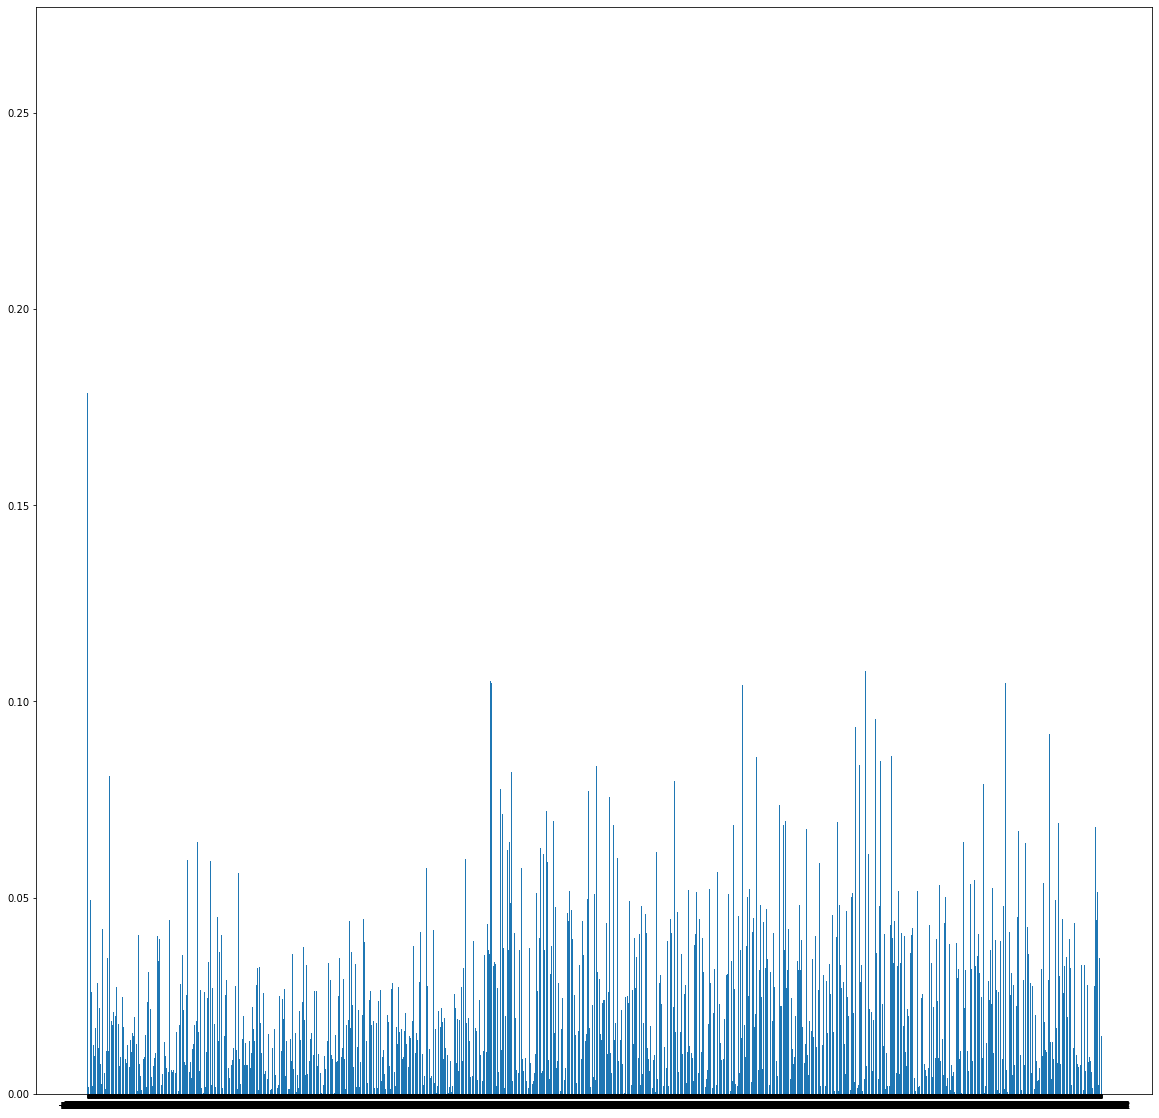
\includegraphics[width=0.75\linewidth]{ipynb/output_44_0.png}
    \caption{The weights including bias learned.}
    \label{fig:weights}
\end{figure}

Fig. \ref{fig:weights} shows the weights that were learned.
The bias is most important in this model.
Most of the weights are equally important,
but there are a few that are more important,
and many more that are not very important and could be reduced.
I did not perform any feature reduction however.

\begin{figure}
    \centering
    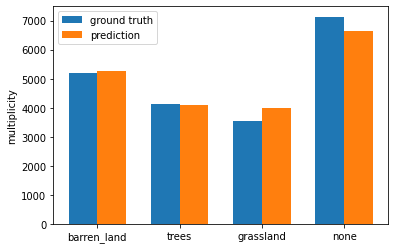
\includegraphics[width=0.75\linewidth]{ipynb/output_52_1.png}
    \caption{Bar plot of the multiplicities of the classes in ground truth and prediction.}
    \label{fig:multiplicity bar plot}
\end{figure}

In Fig. {fig:multiplicity bar plot}, we see a visual representation of the multiplicities of the terrain type classes.
It seems like a close fit.
However, all this is, is a visual representation of a count of each of the classes.

\begin{table}[]
    \centering
    \[
        \begin{array}{@{}llS[round-mode=figures,round-precision=4]@{}}
        \toprule
            \text{dividend} & \text{divisor} & \text{quotient}
        \\*
        \midrule
            \text{MAE train} & \text{MAE test}
            & 0.836726
        \\*
            \text{RMSE train} & \text{RMSE test}
            & 0.843065
        \\*
        \midrule
            \text{MAE test} & \text{MAD train}
            & 0.761874
        \\*
            \text{RMSE test} & \text{\(\sigma\) train}
            & 0.735807
        \\*
        \bottomrule
        \end{array}
    \]
    \caption{Error ratios.}
    \label{tab:error ratios}
\end{table}

Table \ref{tab:error ratios} shows us the results of the linear regression in numbers.
Specifically,
we found that the linear regression was slightly overfit by the two error ratios of \(\num{0.8367}\) and \(\num{0.8431}\).
These represent an overfit because the errors of the training are less than the errors against the test data.
Thus the ratio is less than \(1\).

This table also shows us that the mean absolute error is at about \(0.76\) mean absolute deviations around the median
and that the root mean square error is at about \(0.74\) standard deviations,
which mean that the model has a moderate predictive power since it is close to \(1\).

In their normal forms, mean absolute error and root mean square error give us a measure of the predictive power of the model \cite{rms2016}.
Then
we can use these last two normalizations because the more familiar standard deviation is also known as the root mean square.
In fact, the root mean square error is the same formula as the root mean square,
but using the corresponding predicted value for each label instead of the mean.
Likewise we use the mean absolute deviation about the median to normalize the mean absolute error.

\begin{table}[]
    \centering
    \[
        \begin{array}{@{}SS[round-mode=figures,round-precision=4]l*4{S[round-mode=figures,round-precision=5,group-separator={\,}]}}
        \toprule
            \multicolumn{2}{@{}l}{\text{regularization \(\lambda\)}}
            & \phantom{abc}
            & \text{accuracy}
            & \text{recall}
            & \text{precision}
            & \text{\(F_1\) score}
        \\*
        \cmidrule{1-2}
            \brac*{\si{\deci\bel}}
            &
            \angl{1}
        \\*
        \midrule
            \text{none} &
                && 0.58665
                & 0.4493992231017458
                & 0.6065020921872838
                & 0.5036355376125148
        \\*
        \midrule
            -10 & 0.31622776601683794
                && 0.58715
                & 0.44922446696412854
                & 0.6075849506159723
                & 0.5037411510816644
        \\*
            -9 & 0.35481338923357547
                && 0.5872
                & 0.4492886435781704
                & 0.6077762406861051
                & 0.5038066425016782
        \\*
            -8 & 0.3981071705534972
                && 0.5873
                & 0.4494337852962524
                & 0.607844995207374
                & 0.5039229368765102
        \\*
            -7 & 0.44668359215096315
                && 0.58735
                & 0.4493528201922122
                & 0.6079392009526936
                & 0.5038767122931914
        \\*
            -6 & 0.5011872336272722
                && 0.58735
                & 0.449271855088172
                & 0.6079398509472012
                & 0.5038157451076203
        \\*
        \midrule
            -5 & 0.5623413251903491
                && 0.58755
                & 0.4490842730210176
                & 0.6081144087457719
                & 0.5036484574642933
        \\*
            -4 & 0.6309573444801932
                && 0.5876
                & 0.4490842730210176
                & 0.6083680618451495
                & 0.503697137969315
        \\*
            -3 & 0.7079457843841379
                && 0.58735
                & 0.4486370071517444
                & 0.6078782887164116
                & 0.5031616356837981
        \\*
            -2 & 0.7943282347242815
                && 0.58745
                & 0.44885028804432964
                & 0.6078626211036924
                & 0.5032986730138832
        \\*
            -1 & 0.8912509381337456
                && 0.58755
                & 0.4486755319067122
                & 0.60803368099758
                & 0.5031846728113596
        \\*
        \midrule
            0 & 1.0
                && 0.58775
                & 0.44873970852075407
                & 0.6086427593859304
                & 0.5033432141352383
        \\*
        \midrule
            1 & 1.1220184543019633
                && 0.58775
                & 0.4485649523831367
                & 0.6086225636833118
                & 0.5032103547844932
        \\*
            2 & 1.2589254117941673
                && 0.588
                & 0.448872024309299
                & 0.6090748139440184
                & 0.5035466488795411
        \\*
            3 & 1.4125375446227544
                && 0.5881
                & 0.44869726817168165
                & 0.6095694906461742
                & 0.5035110328600362
        \\*
            4 & 1.5848931924611136
                && 0.5885
                & 0.4487782332757218
                & 0.6104109099997941
                & 0.5037766968830625
        \\*
            5 & 1.7782794100389228
                && 0.5885
                & 0.44852251203406435
                & 0.6107817976750681
                & 0.5036020810947259
        \\*
        \midrule
            6 & 1.9952623149688795
                && 0.58845
                & 0.44817299975882957
                & 0.6107110409285051
                & 0.5032615372821362
        \\*
            7 & 2.2387211385683394
                && 0.58855
                & 0.44798541769167527
                & 0.6107363934997151
                & 0.5030861896774851
        \\*
            8 & 2.51188643150958
                && 0.58875
                & 0.44798541769167527
                & 0.6113871721572975
                & 0.5032827113710475
        \\*
            9 & 2.8183829312644537
                && 0.5891
                & 0.44790445258763506
                & 0.6122752617389601
                & 0.5034322630651811
        \\*
            10 & 3.1622776601683795
                && 0.58925
                & 0.4479094003626063
                & 0.6123493532783794
                & 0.5033598847989803
        \\*
        \bottomrule
        \end{array}
    \]
    \caption{Scores with different values of the regularization hyperparameter \(\lambda\).}
    \label{tab:regularizations scores}
\end{table}

Table \ref{tab:regularizations scores} shows us
the scores for the different regularization hyperparameters \(\lambda\) of a ridge regression
with the first being the original linear regression with no regularization. The models have somewhat bad recall with moderately fair precision. A visiual representation is provided by Fig.\ref{fig:precision vs recall}  below.

\begin{figure}
    \centering
    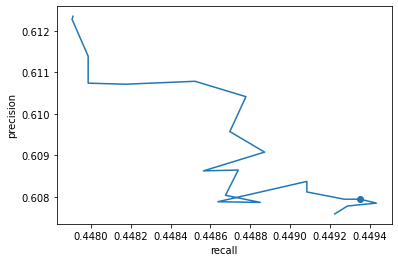
\includegraphics[width=0.75\linewidth]{ipynb/output_67_0.png}
    \caption{Precision versus recall by regularization hyperparameter \(\lambda\) with linear regression as a disc.}
    \label{fig:precision vs recall}
\end{figure}

Hyperparameter
\(\lambda = \SI{-8}{\deci\bel} = 0.3981\)
the \(F_1\) score%
, representing the harmonic mean of recall and precision,
maximizes at \(F_1 = \num[group-separator={\,}]{0.50392}\).

\section{What has been done}

The sampling is working now.
I can now load the datasets,
so it will be possible to work with the sampled datasets now.

\section{What has not been done}

I have not started working on the preprocessing or the model yet.

\section{What will be done during the following week.}

I will do my best to get preprocessing out of the way and do some basic model training and testing.
It will be an iterative process
so I can choose the best minimal model.

\part{Final Project Proposal}

\section{Timeline}
\filbreak
{
    \centering
    \begin{tblr}[%
        long,%
        caption = {Time line}%
    ]{%
        width=0.8667\linewidth,%
        colspec={@{}Xl@{}}%
    }
    \toprule
        Objective & Due Date
    \\*
    \midrule
        data set research & 2022-03-24
    \\*
        initial proposal & 2022-03-25
    \\*
        proposal revising & 2022-04-06
    \\*
        initial data understanding, visualization & 2022-04-06
    \\*
        progress report I revising & 2022-04-06
    \\*
        pre-processing of data & 2022-04-08
    \\*
        progress report II & 2022-04-09
    \\*
        experimenting with logistic regression hyper parameters & 2022-04-15
    \\*
        lightning talks & 2022-04-19
    \\*
        revising presentation of results & 2022-04-22
    \\*
        working on final report & 2022-04-23
    \\*
        \(\prime\prime\)& 2022-04-24
    \\*
    \bottomrule
    \end{tblr}
}
\newpage

\printbibliography

\part{Progress Report I}

\section{What has been done}

I have mostly been working on the sampling.
Because of the limitations of my computer,
I cannot load the entire dataset into memory and perform operations on it.
As a result,
I will instead sample both datasets into \(\num{20000}\) examples
before working with them.

My progress is available at \href{https://github.com/lduran2/CIS3715_DataScience_2022/tree/final/final}{my project repository}.

\section{What has not been done}

I have not started working on the preprocessing or the model yet.

\section{What will be done during the following week.}

I will do my best to get preprocessing out of the way and do some basic model training and testing.
It will be an iterative process
so I can choose the best minimal model.

\newpage
\appendix
\title{CIS 3715 Final Project Report Appendix}

\maketitle

\part{Jupyter notebook of the project}
\graphicspath{{ipynb/}}
    \hypertarget{using-satellite-imagery-to-train-a-model-for-identifying-the-type-of-landmarks}{%
\section{Using satellite imagery to train a model for identifying the
type of
landmarks}\label{using-satellite-imagery-to-train-a-model-for-identifying-the-type-of-landmarks}}

    \hypertarget{preprocess-data}{%
\subsection{Preprocess data}\label{preprocess-data}}

Now we may work with the data.

Start by importing necessary modules and setting up important constants.

    \begin{tcolorbox}[breakable, size=fbox, boxrule=1pt, pad at break*=1mm,colback=cellbackground, colframe=cellborder]
\prompt{In}{incolor}{52}{\boxspacing}
\begin{Verbatim}[commandchars=\\\{\}]
\PY{k+kn}{import} \PY{n+nn}{pandas} \PY{k}{as} \PY{n+nn}{pd}                                         \PY{c+c1}{\PYZsh{} for the dataframes}
\PY{k+kn}{from} \PY{n+nn}{math} \PY{k+kn}{import} \PY{o}{*}                                          \PY{c+c1}{\PYZsh{} for sqrt}
\PY{k+kn}{from} \PY{n+nn}{statistics} \PY{k+kn}{import} \PY{o}{*}                                    \PY{c+c1}{\PYZsh{} for mean}
\PY{k+kn}{import} \PY{n+nn}{numpy} \PY{k}{as} \PY{n+nn}{np}                                          \PY{c+c1}{\PYZsh{} for linear algebra}
\PY{k+kn}{import} \PY{n+nn}{matplotlib}\PY{n+nn}{.}\PY{n+nn}{pyplot} \PY{k}{as} \PY{n+nn}{plt}                             \PY{c+c1}{\PYZsh{} for various plots}
\PY{k+kn}{from} \PY{n+nn}{sklearn}\PY{n+nn}{.}\PY{n+nn}{linear\PYZus{}model} \PY{k+kn}{import} \PY{n}{LinearRegression}\PY{p}{,} \PY{n}{Ridge}    \PY{c+c1}{\PYZsh{} for the learning models}
\PY{k+kn}{from} \PY{n+nn}{sklearn}\PY{n+nn}{.}\PY{n+nn}{metrics} \PY{k+kn}{import} \PYZbs{}
    \PY{n}{mean\PYZus{}absolute\PYZus{}error}\PY{p}{,} \PY{n}{mean\PYZus{}squared\PYZus{}error}                 \PY{c+c1}{\PYZsh{} for evaluating models}
\PY{k+kn}{from} \PY{n+nn}{sklearn}\PY{n+nn}{.}\PY{n+nn}{metrics} \PY{k+kn}{import} \PYZbs{}
    \PY{n}{accuracy\PYZus{}score}\PY{p}{,} \PY{n}{f1\PYZus{}score}\PY{p}{,} \PY{n}{recall\PYZus{}score}\PY{p}{,} \PY{n}{precision\PYZus{}score} \PY{c+c1}{\PYZsh{} for further evaluating models}
\end{Verbatim}
\end{tcolorbox}

    \begin{tcolorbox}[breakable, size=fbox, boxrule=1pt, pad at break*=1mm,colback=cellbackground, colframe=cellborder]
\prompt{In}{incolor}{78}{\boxspacing}
\begin{Verbatim}[commandchars=\\\{\}]
\PY{c+c1}{\PYZsh{} constants}
\PY{n}{X\PYZus{}TRAIN\PYZus{}FILENAME} \PY{o}{=} \PY{l+s+sa}{r}\PY{l+s+s1}{\PYZsq{}}\PY{l+s+s1}{dataset/X\PYZus{}train\PYZus{}sat4\PYZus{}samp20000.csv}\PY{l+s+s1}{\PYZsq{}}    \PY{c+c1}{\PYZsh{} filename of the training dataset input}
\PY{n}{Y\PYZus{}TRAIN\PYZus{}FILENAME} \PY{o}{=} \PY{l+s+sa}{r}\PY{l+s+s1}{\PYZsq{}}\PY{l+s+s1}{dataset/y\PYZus{}train\PYZus{}sat4\PYZus{}samp20000.csv}\PY{l+s+s1}{\PYZsq{}}    \PY{c+c1}{\PYZsh{} filename of the training dataset output}
\PY{n}{X\PYZus{}TEST\PYZus{}FILENAME} \PY{o}{=} \PY{l+s+sa}{r}\PY{l+s+s1}{\PYZsq{}}\PY{l+s+s1}{dataset/X\PYZus{}test\PYZus{}sat4\PYZus{}samp20000.csv}\PY{l+s+s1}{\PYZsq{}}      \PY{c+c1}{\PYZsh{} filename of the testing dataset input}
\PY{n}{Y\PYZus{}TEST\PYZus{}FILENAME} \PY{o}{=} \PY{l+s+sa}{r}\PY{l+s+s1}{\PYZsq{}}\PY{l+s+s1}{dataset/y\PYZus{}test\PYZus{}sat4\PYZus{}samp20000.csv}\PY{l+s+s1}{\PYZsq{}}      \PY{c+c1}{\PYZsh{} filename of the testing dataset output}

\PY{n}{R2\PYZus{}TOLERANCE} \PY{o}{=} \PY{l+m+mf}{0.81}                                         \PY{c+c1}{\PYZsh{} use 0.81 for r\PYZca{}2 for strong correlations}
\PY{n}{ACCURACY\PYZus{}TOLERANCE} \PY{o}{=} \PY{l+m+mf}{0.05}                                   \PY{c+c1}{\PYZsh{} maximum allowed error for accuracy}
\end{Verbatim}
\end{tcolorbox}

    Read in the files and do a high level inspection.

    \begin{tcolorbox}[breakable, size=fbox, boxrule=1pt, pad at break*=1mm,colback=cellbackground, colframe=cellborder]
\prompt{In}{incolor}{3}{\boxspacing}
\begin{Verbatim}[commandchars=\\\{\}]
\PY{c+c1}{\PYZsh{} read in the training data}
\PY{n}{X\PYZus{}train} \PY{o}{=} \PY{n}{pd}\PY{o}{.}\PY{n}{read\PYZus{}csv}\PY{p}{(}\PY{n}{X\PYZus{}TRAIN\PYZus{}FILENAME}\PY{p}{,} \PY{n}{header}\PY{o}{=}\PY{k+kc}{None}\PY{p}{,} \PY{n}{index\PYZus{}col}\PY{o}{=}\PY{k+kc}{None}\PY{p}{)}
\PY{n}{y\PYZus{}train} \PY{o}{=} \PY{n}{pd}\PY{o}{.}\PY{n}{read\PYZus{}csv}\PY{p}{(}\PY{n}{Y\PYZus{}TRAIN\PYZus{}FILENAME}\PY{p}{,} \PY{n}{header}\PY{o}{=}\PY{k+kc}{None}\PY{p}{,} \PY{n}{index\PYZus{}col}\PY{o}{=}\PY{k+kc}{None}\PY{p}{)}
\end{Verbatim}
\end{tcolorbox}

    \begin{tcolorbox}[breakable, size=fbox, boxrule=1pt, pad at break*=1mm,colback=cellbackground, colframe=cellborder]
\prompt{In}{incolor}{4}{\boxspacing}
\begin{Verbatim}[commandchars=\\\{\}]
\PY{c+c1}{\PYZsh{} data shape constants}
\PY{p}{(}\PY{n}{N\PYZus{}XAMPS}\PY{p}{,} \PY{n}{N\PYZus{}FEATS}\PY{p}{)} \PY{o}{=} \PY{n}{X\PYZus{}train}\PY{o}{.}\PY{n}{shape}
\PY{p}{(}\PY{n}{\PYZus{}}\PY{p}{,} \PY{n}{N\PYZus{}LBLS}\PY{p}{)} \PY{o}{=} \PY{n}{y\PYZus{}train}\PY{o}{.}\PY{n}{shape}
\PY{c+c1}{\PYZsh{} colors for grapphing}
\PY{n}{CHANNELS} \PY{o}{=} \PY{p}{(}\PY{l+s+sa}{r}\PY{l+s+s1}{\PYZsq{}}\PY{l+s+s1}{r}\PY{l+s+s1}{\PYZsq{}}\PY{p}{,} \PY{l+s+sa}{r}\PY{l+s+s1}{\PYZsq{}}\PY{l+s+s1}{g}\PY{l+s+s1}{\PYZsq{}}\PY{p}{,} \PY{l+s+sa}{r}\PY{l+s+s1}{\PYZsq{}}\PY{l+s+s1}{b}\PY{l+s+s1}{\PYZsq{}}\PY{p}{,} \PY{l+s+sa}{r}\PY{l+s+s1}{\PYZsq{}}\PY{l+s+s1}{maroon}\PY{l+s+s1}{\PYZsq{}}\PY{p}{)}
\PY{n}{N\PYZus{}CHANNELS} \PY{o}{=} \PY{n+nb}{len}\PY{p}{(}\PY{n}{CHANNELS}\PY{p}{)}
\PY{c+c1}{\PYZsh{} number of pixels}
\PY{n}{NF\PYZus{}PIXELS} \PY{o}{=} \PY{n}{N\PYZus{}FEATS}\PY{o}{/}\PY{n}{N\PYZus{}CHANNELS}
\PY{n}{F\PYZus{}WIDTH} \PY{o}{=} \PY{n}{sqrt}\PY{p}{(}\PY{n}{NF\PYZus{}PIXELS}\PY{p}{)}
\PY{n}{F\PYZus{}HEIGHT} \PY{o}{=} \PY{n}{NF\PYZus{}PIXELS}\PY{o}{/}\PY{n}{F\PYZus{}WIDTH}
\PY{c+c1}{\PYZsh{} round number of pixels}
\PY{n}{NI\PYZus{}PIXELS} \PY{o}{=} \PY{n+nb}{int}\PY{p}{(}\PY{n}{NF\PYZus{}PIXELS}\PY{p}{)}
\PY{n}{I\PYZus{}WIDTH} \PY{o}{=} \PY{n+nb}{int}\PY{p}{(}\PY{n}{F\PYZus{}WIDTH}\PY{p}{)}
\PY{n}{I\PYZus{}HEIGHT} \PY{o}{=} \PY{n+nb}{int}\PY{p}{(}\PY{n}{F\PYZus{}HEIGHT}\PY{p}{)}

\PY{n+nb}{print}\PY{p}{(}\PY{l+s+sa}{r}\PY{l+s+s2}{\PYZdq{}}\PY{l+s+si}{\PYZob{}\PYZcb{}}\PY{l+s+s2}{ images of (}\PY{l+s+si}{\PYZob{}\PYZcb{}}\PY{l+s+s2}{x}\PY{l+s+si}{\PYZob{}\PYZcb{}}\PY{l+s+s2}{)px x }\PY{l+s+si}{\PYZob{}\PYZcb{}}\PY{l+s+s2}{ channels}\PY{l+s+s2}{\PYZdq{}}\PY{o}{.}\PY{n}{format}\PY{p}{(}\PY{n}{N\PYZus{}XAMPS}\PY{p}{,} \PY{n}{I\PYZus{}WIDTH}\PY{p}{,} \PY{n}{I\PYZus{}HEIGHT}\PY{p}{,} \PY{n}{N\PYZus{}CHANNELS}\PY{p}{)}\PY{p}{)}
\end{Verbatim}
\end{tcolorbox}

    \begin{Verbatim}[commandchars=\\\{\}]
20000 images of (28x28)px x 4 channels
    \end{Verbatim}

    \begin{tcolorbox}[breakable, size=fbox, boxrule=1pt, pad at break*=1mm,colback=cellbackground, colframe=cellborder]
\prompt{In}{incolor}{5}{\boxspacing}
\begin{Verbatim}[commandchars=\\\{\}]
\PY{c+c1}{\PYZsh{} combine training data features, labels}
\PY{n}{df\PYZus{}train} \PY{o}{=} \PY{n}{pd}\PY{o}{.}\PY{n}{concat}\PY{p}{(}\PY{p}{[}\PY{n}{X\PYZus{}train}\PY{p}{,} \PY{n}{y\PYZus{}train}\PY{p}{]}\PY{p}{,} \PY{n}{axis}\PY{o}{=}\PY{l+m+mi}{1}\PY{p}{)}
\end{Verbatim}
\end{tcolorbox}

    \begin{tcolorbox}[breakable, size=fbox, boxrule=1pt, pad at break*=1mm,colback=cellbackground, colframe=cellborder]
\prompt{In}{incolor}{6}{\boxspacing}
\begin{Verbatim}[commandchars=\\\{\}]
\PY{c+c1}{\PYZsh{} print shapes of X, y}
\PY{n+nb}{print}\PY{p}{(}\PY{l+s+s2}{\PYZdq{}}\PY{l+s+s2}{X\PYZus{}train shape}\PY{l+s+se}{\PYZbs{}t}\PY{l+s+si}{\PYZob{}\PYZcb{}}\PY{l+s+s2}{\PYZdq{}}\PY{o}{.}\PY{n}{format}\PY{p}{(}\PY{n}{X\PYZus{}train}\PY{o}{.}\PY{n}{shape}\PY{p}{)}\PY{p}{)}
\PY{n+nb}{print}\PY{p}{(}\PY{l+s+s2}{\PYZdq{}}\PY{l+s+s2}{y\PYZus{}train shape}\PY{l+s+se}{\PYZbs{}t}\PY{l+s+si}{\PYZob{}\PYZcb{}}\PY{l+s+s2}{\PYZdq{}}\PY{o}{.}\PY{n}{format}\PY{p}{(}\PY{n}{y\PYZus{}train}\PY{o}{.}\PY{n}{shape}\PY{p}{)}\PY{p}{)}
\PY{n+nb}{print}\PY{p}{(}\PY{l+s+s2}{\PYZdq{}}\PY{l+s+s2}{combined shape}\PY{l+s+se}{\PYZbs{}t}\PY{l+s+si}{\PYZob{}\PYZcb{}}\PY{l+s+s2}{\PYZdq{}}\PY{o}{.}\PY{n}{format}\PY{p}{(}\PY{n}{df\PYZus{}train}\PY{o}{.}\PY{n}{shape}\PY{p}{)}\PY{p}{)}
\end{Verbatim}
\end{tcolorbox}

    \begin{Verbatim}[commandchars=\\\{\}]
X\_train shape   (20000, 3136)
y\_train shape   (20000, 4)
combined shape  (20000, 3140)
    \end{Verbatim}

    \begin{tcolorbox}[breakable, size=fbox, boxrule=1pt, pad at break*=1mm,colback=cellbackground, colframe=cellborder]
\prompt{In}{incolor}{7}{\boxspacing}
\begin{Verbatim}[commandchars=\\\{\}]
\PY{c+c1}{\PYZsh{} print some basic information about the dataset}
\PY{n+nb}{print}\PY{p}{(}\PY{l+s+s1}{\PYZsq{}}\PY{l+s+se}{\PYZbs{}n}\PY{l+s+s1}{===data frame information===}\PY{l+s+s1}{\PYZsq{}}\PY{p}{)}
\PY{n}{df\PYZus{}train}\PY{o}{.}\PY{n}{info}\PY{p}{(}\PY{p}{)}

\PY{c+c1}{\PYZsh{} print its parameters}
\PY{n+nb}{print}\PY{p}{(}\PY{l+s+s1}{\PYZsq{}}\PY{l+s+se}{\PYZbs{}n}\PY{l+s+s1}{===data frame parameters===}\PY{l+s+s1}{\PYZsq{}}\PY{p}{)}
\PY{n}{df\PYZus{}train}\PY{o}{.}\PY{n}{describe}\PY{p}{(}\PY{p}{)}
\end{Verbatim}
\end{tcolorbox}

    \begin{Verbatim}[commandchars=\\\{\}]

===data frame information===
<class 'pandas.core.frame.DataFrame'>
RangeIndex: 20000 entries, 0 to 19999
Columns: 3140 entries, 0 to 3
dtypes: int64(3140)
memory usage: 479.1 MB

===data frame parameters===
    \end{Verbatim}

            \begin{tcolorbox}[breakable, size=fbox, boxrule=.5pt, pad at break*=1mm, opacityfill=0]
\prompt{Out}{outcolor}{7}{\boxspacing}
\begin{Verbatim}[commandchars=\\\{\}]
               0             1             2             3             4     \textbackslash{}
count  20000.000000  20000.000000  20000.000000  20000.000000  20000.000000
mean     127.778700    123.954900    110.979800    158.810900    127.608900
std       42.825413     37.944932     35.705831     37.819527     42.946379
min        0.000000      3.000000      1.000000      4.000000      0.000000
25\%       98.000000     99.000000     89.000000    140.000000     98.000000
50\%      124.000000    122.000000    110.000000    166.000000    123.000000
75\%      159.000000    148.000000    132.000000    185.000000    159.000000
max      255.000000    255.000000    255.000000    253.000000    244.000000

              5             6             7             8             9     \textbackslash{}
count  20000.00000  20000.000000  20000.000000  20000.000000  20000.000000
mean     123.83680    110.863550    158.690150    127.607600    123.907450
std       38.08994     35.786297     37.861817     42.864149     37.943326
min        2.00000      0.000000      0.000000      0.000000      1.000000
25\%       99.00000     89.000000    140.000000     98.000000     99.000000
50\%      122.00000    109.000000    166.000000    123.000000    122.000000
75\%      148.00000    132.000000    185.000000    158.000000    148.000000
max      255.00000    255.000000    252.000000    246.000000    255.000000

       {\ldots}          3130          3131          3132          3133  \textbackslash{}
count  {\ldots}  20000.000000  20000.000000  20000.000000  20000.000000
mean   {\ldots}    111.151800    158.804500    128.173150    124.216950
std    {\ldots}     35.980267     37.691749     42.905264     37.907691
min    {\ldots}      0.000000      0.000000      0.000000      2.000000
25\%    {\ldots}     89.000000    140.000000     99.000000    100.000000
50\%    {\ldots}    110.000000    166.000000    124.000000    122.000000
75\%    {\ldots}    133.000000    185.000000    159.000000    148.000000
max    {\ldots}    255.000000    254.000000    248.000000    251.000000

              3134         3135          0             1             2     \textbackslash{}
count  20000.00000  20000.00000  20000.000000  20000.000000  20000.000000
mean     111.20020    158.91350      0.263800      0.201600      0.178600
std       35.64033     37.59736      0.440703      0.401205      0.383027
min        0.00000      3.00000      0.000000      0.000000      0.000000
25\%       89.00000    140.00000      0.000000      0.000000      0.000000
50\%      110.00000    166.00000      0.000000      0.000000      0.000000
75\%      133.00000    185.00000      1.000000      0.000000      0.000000
max      255.00000    245.00000      1.000000      1.000000      1.000000

               3
count  20000.000000
mean       0.356000
std        0.478827
min        0.000000
25\%        0.000000
50\%        0.000000
75\%        1.000000
max        1.000000

[8 rows x 3140 columns]
\end{Verbatim}
\end{tcolorbox}
        
    We can see from these summaries that all \(3140\) columns, features and
labels, are \texttt{int64}, and thus numerical features.

    \begin{tcolorbox}[breakable, size=fbox, boxrule=1pt, pad at break*=1mm,colback=cellbackground, colframe=cellborder]
\prompt{In}{incolor}{8}{\boxspacing}
\begin{Verbatim}[commandchars=\\\{\}]
\PY{c+c1}{\PYZsh{} calculate the number of missing values}
\PY{n}{n\PYZus{}missing} \PY{o}{=} \PY{n}{df\PYZus{}train}\PY{o}{.}\PY{n}{isnull}\PY{p}{(}\PY{p}{)}\PY{o}{.}\PY{n}{sum}\PY{p}{(}\PY{p}{)}

\PY{c+c1}{\PYZsh{} print the number missing for each column,}
\PY{c+c1}{\PYZsh{} but ignore 0s since there are so many columns}
\PY{n+nb}{print}\PY{p}{(}\PY{l+s+sa}{r}\PY{l+s+s1}{\PYZsq{}}\PY{l+s+s1}{===\PYZsh{} missing values per column===}\PY{l+s+s1}{\PYZsq{}}\PY{p}{)}
\PY{n+nb}{print}\PY{p}{(}\PY{n}{n\PYZus{}missing}\PY{p}{[}\PY{n}{n\PYZus{}missing} \PY{o}{!=} \PY{l+m+mi}{0}\PY{p}{]}\PY{p}{)}
\end{Verbatim}
\end{tcolorbox}

    \begin{Verbatim}[commandchars=\\\{\}]
===\# missing values per column===
Series([], dtype: int64)
    \end{Verbatim}

    Additionally, we find that there are no columns with missing values.
Let's inspect the distributions of each feature and the label.

    Since there are so many features (\(3136\)), we will plot the skewness
of each feature by pixel row, rather than a histogram.

    \begin{tcolorbox}[breakable, size=fbox, boxrule=1pt, pad at break*=1mm,colback=cellbackground, colframe=cellborder]
\prompt{In}{incolor}{9}{\boxspacing}
\begin{Verbatim}[commandchars=\\\{\}]
\PY{c+c1}{\PYZsh{} centralize the data frame}
\PY{n}{central\PYZus{}X} \PY{o}{=} \PY{n}{X\PYZus{}train} \PY{o}{\PYZhy{}} \PY{n}{X\PYZus{}train}\PY{o}{.}\PY{n}{mean}\PY{p}{(}\PY{p}{)}
\PY{c+c1}{\PYZsh{} calculate standard deviations}
\PY{n}{X\PYZus{}std} \PY{o}{=} \PY{n}{X\PYZus{}train}\PY{o}{.}\PY{n}{std}\PY{p}{(}\PY{p}{)}
\PY{c+c1}{\PYZsh{} calculate the skews of each column}
\PY{n}{skews} \PY{o}{=} \PY{n}{N\PYZus{}XAMPS}\PY{o}{*}\PY{p}{(}\PY{n}{central\PYZus{}X}\PY{o}{*}\PY{o}{*}\PY{l+m+mi}{3}\PY{p}{)}\PY{o}{.}\PY{n}{sum}\PY{p}{(}\PY{p}{)}\PY{o}{/}\PY{p}{(}\PY{p}{(}\PY{n}{N\PYZus{}XAMPS} \PY{o}{\PYZhy{}} \PY{l+m+mi}{1}\PY{p}{)}\PY{o}{*}\PY{p}{(}\PY{n}{N\PYZus{}XAMPS} \PY{o}{\PYZhy{}} \PY{l+m+mi}{2}\PY{p}{)}\PY{o}{*}\PY{n}{X\PYZus{}std}\PY{o}{*}\PY{o}{*}\PY{l+m+mi}{3}\PY{p}{)}
\end{Verbatim}
\end{tcolorbox}

    \begin{tcolorbox}[breakable, size=fbox, boxrule=1pt, pad at break*=1mm,colback=cellbackground, colframe=cellborder]
\prompt{In}{incolor}{10}{\boxspacing}
\begin{Verbatim}[commandchars=\\\{\}]
\PY{c+c1}{\PYZsh{} let\PYZsq{}s scatter graph the features}
\PY{c+c1}{\PYZsh{} 28x28, color code RGB}
\PY{c+c1}{\PYZsh{} x\PYZsq{}s in scatter graph}
\PY{n}{scatter\PYZus{}x} \PY{o}{=} \PY{n+nb}{sum}\PY{p}{(}\PY{p}{(}\PY{p}{[}\PY{n}{k}\PY{p}{]}\PY{o}{*}\PY{n}{N\PYZus{}CHANNELS} \PY{k}{for} \PY{n}{k} \PY{o+ow}{in} \PY{n+nb}{range}\PY{p}{(}\PY{n}{I\PYZus{}WIDTH}\PY{p}{)}\PY{p}{)}\PY{p}{,} \PY{p}{[}\PY{p}{]}\PY{p}{)}
\PY{c+c1}{\PYZsh{} colors for the scatter graph}
\PY{n}{scatter\PYZus{}colors} \PY{o}{=} \PY{p}{(}\PY{n}{CHANNELS}\PY{o}{*}\PY{n}{I\PYZus{}WIDTH}\PY{p}{)}
\PY{c+c1}{\PYZsh{} its size}
\PY{n}{ROW\PYZus{}SIZE} \PY{o}{=} \PY{p}{(}\PY{n}{N\PYZus{}CHANNELS}\PY{o}{*}\PY{n}{I\PYZus{}WIDTH}\PY{p}{)}

\PY{c+c1}{\PYZsh{} loop through pixel rows}
\PY{k}{for} \PY{n}{i\PYZus{}row} \PY{o+ow}{in} \PY{n+nb}{range}\PY{p}{(}\PY{l+m+mi}{0}\PY{p}{,} \PY{n}{I\PYZus{}HEIGHT}\PY{p}{)}\PY{p}{:}
    \PY{c+c1}{\PYZsh{} offset in data frame for this row}
    \PY{n}{offset} \PY{o}{=} \PY{p}{(}\PY{n}{i\PYZus{}row}\PY{o}{*}\PY{n}{ROW\PYZus{}SIZE}\PY{p}{)}
    \PY{c+c1}{\PYZsh{} create the row as a list}
    \PY{n}{row} \PY{o}{=} \PY{n+nb}{list}\PY{p}{(}\PY{n}{skews}\PY{p}{[}\PY{n}{X\PYZus{}train}\PY{o}{.}\PY{n}{columns}\PY{p}{[}\PY{n}{offset}\PY{p}{:}\PY{p}{(}\PY{n}{offset} \PY{o}{+} \PY{n}{ROW\PYZus{}SIZE}\PY{p}{)}\PY{p}{]}\PY{p}{]}\PY{p}{)}
    \PY{c+c1}{\PYZsh{} plot the row}
    \PY{n}{plt}\PY{o}{.}\PY{n}{scatter}\PY{p}{(}\PY{n}{scatter\PYZus{}x}\PY{p}{,} \PY{n}{row}\PY{p}{,} \PY{n}{c}\PY{o}{=}\PY{n}{scatter\PYZus{}colors}\PY{p}{,} \PY{n}{marker}\PY{o}{=}\PY{l+s+s1}{\PYZsq{}}\PY{l+s+s1}{x}\PY{l+s+s1}{\PYZsq{}}\PY{p}{)}
    \PY{n}{plt}\PY{o}{.}\PY{n}{ylabel}\PY{p}{(}\PY{l+s+s2}{\PYZdq{}}\PY{l+s+s2}{row }\PY{l+s+si}{\PYZob{}\PYZcb{}}\PY{l+s+s2}{\PYZdq{}}\PY{o}{.}\PY{n}{format}\PY{p}{(}\PY{n}{i\PYZus{}row}\PY{p}{)}\PY{p}{)}
    \PY{n}{plt}\PY{o}{.}\PY{n}{show}\PY{p}{(}\PY{p}{)}
\PY{c+c1}{\PYZsh{} next i\PYZus{}row}
\end{Verbatim}
\end{tcolorbox}

    \begin{center}
    \adjustimage{max size={0.9\linewidth}{0.9\paperheight}}{output_18_0.png}
    \end{center}
    { \hspace*{\fill} \\}
    
    \begin{center}
    \adjustimage{max size={0.9\linewidth}{0.9\paperheight}}{output_18_1.png}
    \end{center}
    { \hspace*{\fill} \\}
    
    \begin{center}
    \adjustimage{max size={0.9\linewidth}{0.9\paperheight}}{output_18_2.png}
    \end{center}
    { \hspace*{\fill} \\}
    
    \begin{center}
    \adjustimage{max size={0.9\linewidth}{0.9\paperheight}}{output_18_3.png}
    \end{center}
    { \hspace*{\fill} \\}
    
    \begin{center}
    \adjustimage{max size={0.9\linewidth}{0.9\paperheight}}{output_18_4.png}
    \end{center}
    { \hspace*{\fill} \\}
    
    \begin{center}
    \adjustimage{max size={0.9\linewidth}{0.9\paperheight}}{output_18_5.png}
    \end{center}
    { \hspace*{\fill} \\}
    
    \begin{center}
    \adjustimage{max size={0.9\linewidth}{0.9\paperheight}}{output_18_6.png}
    \end{center}
    { \hspace*{\fill} \\}
    
    \begin{center}
    \adjustimage{max size={0.9\linewidth}{0.9\paperheight}}{output_18_7.png}
    \end{center}
    { \hspace*{\fill} \\}
    
    \begin{center}
    \adjustimage{max size={0.9\linewidth}{0.9\paperheight}}{output_18_8.png}
    \end{center}
    { \hspace*{\fill} \\}
    
    \begin{center}
    \adjustimage{max size={0.9\linewidth}{0.9\paperheight}}{output_18_9.png}
    \end{center}
    { \hspace*{\fill} \\}
    
    \begin{center}
    \adjustimage{max size={0.9\linewidth}{0.9\paperheight}}{output_18_10.png}
    \end{center}
    { \hspace*{\fill} \\}
    
    \begin{center}
    \adjustimage{max size={0.9\linewidth}{0.9\paperheight}}{output_18_11.png}
    \end{center}
    { \hspace*{\fill} \\}
    
    \begin{center}
    \adjustimage{max size={0.9\linewidth}{0.9\paperheight}}{output_18_12.png}
    \end{center}
    { \hspace*{\fill} \\}
    
    \begin{center}
    \adjustimage{max size={0.9\linewidth}{0.9\paperheight}}{output_18_13.png}
    \end{center}
    { \hspace*{\fill} \\}
    
    \begin{center}
    \adjustimage{max size={0.9\linewidth}{0.9\paperheight}}{output_18_14.png}
    \end{center}
    { \hspace*{\fill} \\}
    
    \begin{center}
    \adjustimage{max size={0.9\linewidth}{0.9\paperheight}}{output_18_15.png}
    \end{center}
    { \hspace*{\fill} \\}
    
    \begin{center}
    \adjustimage{max size={0.9\linewidth}{0.9\paperheight}}{output_18_16.png}
    \end{center}
    { \hspace*{\fill} \\}
    
    \begin{center}
    \adjustimage{max size={0.9\linewidth}{0.9\paperheight}}{output_18_17.png}
    \end{center}
    { \hspace*{\fill} \\}
    
    \begin{center}
    \adjustimage{max size={0.9\linewidth}{0.9\paperheight}}{output_18_18.png}
    \end{center}
    { \hspace*{\fill} \\}
    
    \begin{center}
    \adjustimage{max size={0.9\linewidth}{0.9\paperheight}}{output_18_19.png}
    \end{center}
    { \hspace*{\fill} \\}
    
    \begin{center}
    \adjustimage{max size={0.9\linewidth}{0.9\paperheight}}{output_18_20.png}
    \end{center}
    { \hspace*{\fill} \\}
    
    \begin{center}
    \adjustimage{max size={0.9\linewidth}{0.9\paperheight}}{output_18_21.png}
    \end{center}
    { \hspace*{\fill} \\}
    
    \begin{center}
    \adjustimage{max size={0.9\linewidth}{0.9\paperheight}}{output_18_22.png}
    \end{center}
    { \hspace*{\fill} \\}
    
    \begin{center}
    \adjustimage{max size={0.9\linewidth}{0.9\paperheight}}{output_18_23.png}
    \end{center}
    { \hspace*{\fill} \\}
    
    \begin{center}
    \adjustimage{max size={0.9\linewidth}{0.9\paperheight}}{output_18_24.png}
    \end{center}
    { \hspace*{\fill} \\}
    
    \begin{center}
    \adjustimage{max size={0.9\linewidth}{0.9\paperheight}}{output_18_25.png}
    \end{center}
    { \hspace*{\fill} \\}
    
    \begin{center}
    \adjustimage{max size={0.9\linewidth}{0.9\paperheight}}{output_18_26.png}
    \end{center}
    { \hspace*{\fill} \\}
    
    \begin{center}
    \adjustimage{max size={0.9\linewidth}{0.9\paperheight}}{output_18_27.png}
    \end{center}
    { \hspace*{\fill} \\}
    
    We can see from these scatter plots that: * the red, green and blue
channel are consistently approximately semetric (\(\in [-0.5, 0.5]\))
(especially the red and green colors). Thus they are non-long tail
distributions. * the near infrared (NIR) channel are consistently highly
skewed negative (\(\in [-\infty,-1.0]\)). Thus this is a long tail
distribution.

Therefore, if there were missing values for us to replace, we would use
the mean for the red, green and blue channels, and the median for the
NIR channel.

    Next, we see the correlations to find any features that we can remove.

    \begin{tcolorbox}[breakable, size=fbox, boxrule=1pt, pad at break*=1mm,colback=cellbackground, colframe=cellborder]
\prompt{In}{incolor}{11}{\boxspacing}
\begin{Verbatim}[commandchars=\\\{\}]
\PY{c+c1}{\PYZsh{} calculate the square correlations}
\PY{n}{X\PYZus{}cor2} \PY{o}{=} \PY{n}{X\PYZus{}train}\PY{o}{.}\PY{n}{cov}\PY{p}{(}\PY{p}{)}\PY{o}{*}\PY{o}{*}\PY{l+m+mi}{2}
\PY{n}{X\PYZus{}var} \PY{o}{=} \PY{n}{X\PYZus{}std}\PY{o}{*}\PY{o}{*}\PY{l+m+mi}{2}
\PY{n}{X\PYZus{}varprod} \PY{o}{=} \PY{n}{pd}\PY{o}{.}\PY{n}{DataFrame}\PY{p}{(}\PY{p}{[}\PY{p}{(}\PY{n}{v0}\PY{o}{*}\PY{n}{v1}\PY{p}{)} \PY{k}{for} \PY{n}{v1} \PY{o+ow}{in} \PY{n}{X\PYZus{}var}\PY{p}{]} \PY{k}{for} \PY{n}{v0} \PY{o+ow}{in} \PY{n}{X\PYZus{}var}\PY{p}{)}
\PY{c+c1}{\PYZsh{} normalize X\PYZus{}cor2 using the product of the corresponding variances}
\PY{n}{X\PYZus{}cor2} \PY{o}{=} \PY{p}{(}\PY{n}{X\PYZus{}cor2} \PY{o}{/} \PY{n}{X\PYZus{}varprod}\PY{p}{)}
\end{Verbatim}
\end{tcolorbox}

    \begin{tcolorbox}[breakable, size=fbox, boxrule=1pt, pad at break*=1mm,colback=cellbackground, colframe=cellborder]
\prompt{In}{incolor}{12}{\boxspacing}
\begin{Verbatim}[commandchars=\\\{\}]
\PY{c+c1}{\PYZsh{} find strong correlations}
\PY{n}{is\PYZus{}strong\PYZus{}corr} \PY{o}{=} \PY{p}{(}\PY{n}{X\PYZus{}cor2} \PY{o}{\PYZgt{}}\PY{o}{=} \PY{n}{R2\PYZus{}TOLERANCE}\PY{p}{)}
\PY{c+c1}{\PYZsh{} graph results}
\PY{n}{plt}\PY{o}{.}\PY{n}{figure}\PY{p}{(}\PY{n}{figsize}\PY{o}{=}\PY{p}{(}\PY{l+m+mi}{20}\PY{p}{,} \PY{l+m+mi}{20}\PY{p}{)}\PY{p}{)}
\PY{n}{plt}\PY{o}{.}\PY{n}{imshow}\PY{p}{(}\PY{n}{is\PYZus{}strong\PYZus{}corr}\PY{p}{,} \PY{n}{cmap}\PY{o}{=}\PY{l+s+s1}{\PYZsq{}}\PY{l+s+s1}{PuBu}\PY{l+s+s1}{\PYZsq{}}\PY{p}{)}
\PY{n}{plt}\PY{o}{.}\PY{n}{show}\PY{p}{(}\PY{p}{)}
\end{Verbatim}
\end{tcolorbox}

    \begin{center}
    \adjustimage{max size={0.9\linewidth}{0.9\paperheight}}{output_22_0.png}
    \end{center}
    { \hspace*{\fill} \\}
    
    \begin{tcolorbox}[breakable, size=fbox, boxrule=1pt, pad at break*=1mm,colback=cellbackground, colframe=cellborder]
\prompt{In}{incolor}{13}{\boxspacing}
\begin{Verbatim}[commandchars=\\\{\}]
\PY{c+c1}{\PYZsh{} create a table of the strong correlations per feature}
\PY{n}{i\PYZus{}strong\PYZus{}corr\PYZus{}per\PYZus{}feat} \PY{o}{=} \PY{n}{pd}\PY{o}{.}\PY{n}{DataFrame}\PY{p}{(}\PY{n}{is\PYZus{}strong\PYZus{}corr}\PY{p}{[}\PY{n}{k}\PY{p}{]}\PY{o}{.}\PY{n}{to\PYZus{}numpy}\PY{p}{(}\PY{p}{)}\PY{o}{.}\PY{n}{nonzero}\PY{p}{(}\PY{p}{)} \PY{k}{for} \PY{n}{k} \PY{o+ow}{in} \PY{n+nb}{range}\PY{p}{(}\PY{n}{N\PYZus{}FEATS}\PY{p}{)}\PY{p}{)}
\PY{n}{i\PYZus{}strong\PYZus{}corr\PYZus{}per\PYZus{}feat}
\end{Verbatim}
\end{tcolorbox}

            \begin{tcolorbox}[breakable, size=fbox, boxrule=.5pt, pad at break*=1mm, opacityfill=0]
\prompt{Out}{outcolor}{13}{\boxspacing}
\begin{Verbatim}[commandchars=\\\{\}]
                                         0
0                      [0, 1, 4, 112, 116]
1                                [0, 1, 2]
2                                   [1, 2]
3                                 [3, 115]
4              [0, 4, 5, 8, 112, 116, 120]
{\ldots}                                    {\ldots}
3131                          [3019, 3131]
3132  [3016, 3020, 3128, 3132, 3133, 3134]
3133                    [3132, 3133, 3134]
3134                    [3132, 3133, 3134]
3135                          [3023, 3135]

[3136 rows x 1 columns]
\end{Verbatim}
\end{tcolorbox}
        
    Going by domain knowledge of the features, we know that they are all
linearly independent.

    There seem to be strong correlations at about \(112\) flattened pixels
from each pixel in either direction of most pixels corresponding to
\(112\,\text{px} \times \frac{1\,\text{row}}{28\,\text{px}} = 4\,\text{rows}\)
up or down respectively. However, it was not consistent enough to rely
on for reducing dimensionality.

    Finally, the labels are one-hot encoded, representing

\begin{longtable}[]{@{}lrrrr@{}}
\toprule
terrain type & \texttt{1000} & \texttt{0100} & \texttt{0010} &
\texttt{0001} \\
\midrule
\endhead
\texttt{barren\_land} & 1 & 0 & 0 & 0 \\
\texttt{trees} & 0 & 1 & 0 & 0 \\
\texttt{grassland} & 0 & 0 & 1 & 0 \\
\texttt{none} & 0 & 0 & 0 & 1 \\
\bottomrule
\end{longtable}

Now to see how balanced the target data is, we use a bar plot.

    \begin{tcolorbox}[breakable, size=fbox, boxrule=1pt, pad at break*=1mm,colback=cellbackground, colframe=cellborder]
\prompt{In}{incolor}{14}{\boxspacing}
\begin{Verbatim}[commandchars=\\\{\}]
\PY{c+c1}{\PYZsh{} find the label and its label counts}
\PY{n}{y\PYZus{}train\PYZus{}counts} \PY{o}{=} \PY{n}{y\PYZus{}train}\PY{o}{.}\PY{n}{value\PYZus{}counts}\PY{p}{(}\PY{p}{)}
\PY{n}{r\PYZus{}diff} \PY{o}{=} \PY{l+m+mi}{2}\PY{o}{*}\PY{n+nb}{abs}\PY{p}{(}\PY{n}{y\PYZus{}train\PYZus{}counts}\PY{p}{[}\PY{l+m+mi}{0}\PY{p}{]} \PY{o}{\PYZhy{}} \PY{n}{y\PYZus{}train\PYZus{}counts}\PY{p}{[}\PY{l+m+mi}{1}\PY{p}{]}\PY{p}{)}\PY{o}{/}\PY{p}{(}\PY{n}{y\PYZus{}train\PYZus{}counts}\PY{p}{[}\PY{l+m+mi}{0}\PY{p}{]} \PY{o}{+} \PY{n}{y\PYZus{}train\PYZus{}counts}\PY{p}{[}\PY{l+m+mi}{1}\PY{p}{]}\PY{p}{)}

\PY{c+c1}{\PYZsh{} print and bar plot of the label}
\PY{n+nb}{print}\PY{p}{(}\PY{l+s+sa}{r}\PY{l+s+s1}{\PYZsq{}}\PY{l+s+s1}{===y\PYZus{}train===}\PY{l+s+s1}{\PYZsq{}}\PY{p}{)}
\PY{n+nb}{print}\PY{p}{(}\PY{n}{y\PYZus{}train}\PY{p}{)}
\PY{n+nb}{print}\PY{p}{(}\PY{p}{)}
\PY{n+nb}{print}\PY{p}{(}\PY{l+s+sa}{r}\PY{l+s+s1}{\PYZsq{}}\PY{l+s+s1}{===value counts===}\PY{l+s+s1}{\PYZsq{}}\PY{p}{)}
\PY{n+nb}{print}\PY{p}{(}\PY{n}{y\PYZus{}train\PYZus{}counts}\PY{p}{)}
\PY{n+nb}{print}\PY{p}{(}\PY{p}{)}
\PY{n+nb}{print}\PY{p}{(}\PY{l+s+sa}{r}\PY{l+s+s2}{\PYZdq{}}\PY{l+s+s2}{rate of difference = }\PY{l+s+si}{\PYZob{}\PYZcb{}}\PY{l+s+s2}{\PYZdq{}}\PY{o}{.}\PY{n}{format}\PY{p}{(}\PY{n}{r\PYZus{}diff}\PY{p}{)}\PY{p}{)}
\PY{n}{y\PYZus{}train\PYZus{}counts}\PY{o}{.}\PY{n}{plot}\PY{p}{(}\PY{n}{kind}\PY{o}{=}\PY{l+s+sa}{r}\PY{l+s+s1}{\PYZsq{}}\PY{l+s+s1}{bar}\PY{l+s+s1}{\PYZsq{}}\PY{p}{)}
\PY{n}{plt}\PY{o}{.}\PY{n}{show}\PY{p}{(}\PY{p}{)}
\end{Verbatim}
\end{tcolorbox}

    \begin{Verbatim}[commandchars=\\\{\}]
===y\_train===
       0  1  2  3
0      0  1  0  0
1      1  0  0  0
2      0  0  0  1
3      1  0  0  0
4      1  0  0  0
{\ldots}   .. .. .. ..
19995  0  0  1  0
19996  1  0  0  0
19997  1  0  0  0
19998  0  1  0  0
19999  0  0  1  0

[20000 rows x 4 columns]

===value counts===
0  1  2  3
0  0  0  1    7120
1  0  0  0    5276
0  1  0  0    4032
   0  1  0    3572
dtype: int64

rate of difference = 1  2  3
0  0  0   NaN
      1   NaN
   1  0   NaN
1  0  0   NaN
dtype: float64
    \end{Verbatim}

    \begin{center}
    \adjustimage{max size={0.9\linewidth}{0.9\paperheight}}{output_27_1.png}
    \end{center}
    { \hspace*{\fill} \\}
    
    We see that these total

\[
    \begin{array}{@{}rr@{}}
    \hline
        \text{encoding} & \text{multiplicity}
    \\
    \hline
        1000            &  5276
    \\
        0100            &  4032
    \\
        0010            &  3572
    \\
        0001            &  7120
    \\
    \hline
        \sum            & 20000\rlap.
    \\
    \hline
    \end{array}
\]

Now consider that we have a vector \(\vec{v}\) of \(4\) Boolean
integers. Well in our case, \[
    \mathbf{1}_4^\intercal
    \mathbf{v}
    = 1.
\]

Thus for any order, it is the case that \(v_4 = 1 - (v_1 + v_2 + v_3)\).
Therefore, we can remove one of these label columns and have a linearly
independent set of columns. I choose to remove \texttt{0001} because it
is the last column.

    \begin{tcolorbox}[breakable, size=fbox, boxrule=1pt, pad at break*=1mm,colback=cellbackground, colframe=cellborder]
\prompt{In}{incolor}{15}{\boxspacing}
\begin{Verbatim}[commandchars=\\\{\}]
\PY{c+c1}{\PYZsh{} columns to keep for linear independence}
\PY{n}{y\PYZus{}lind\PYZus{}cols} \PY{o}{=} \PY{n}{y\PYZus{}train}\PY{o}{.}\PY{n}{columns}\PY{p}{[}\PY{l+m+mi}{0}\PY{p}{:}\PY{o}{\PYZhy{}}\PY{l+m+mi}{1}\PY{p}{]}
\PY{c+c1}{\PYZsh{} remove the last column of the the labels}
\PY{n}{y\PYZus{}train\PYZus{}lind} \PY{o}{=} \PY{n}{y\PYZus{}train}\PY{p}{[}\PY{n}{y\PYZus{}lind\PYZus{}cols}\PY{p}{]}
\PY{c+c1}{\PYZsh{} confirm the removal}
\PY{n+nb}{print}\PY{p}{(}\PY{n}{y\PYZus{}train\PYZus{}lind}\PY{o}{.}\PY{n}{shape}\PY{p}{)}
\end{Verbatim}
\end{tcolorbox}

    \begin{Verbatim}[commandchars=\\\{\}]
(20000, 3)
    \end{Verbatim}

    \hypertarget{split-the-data-and-normalize-the-features-of-examples-according-to-training-data}{%
\subsection{Split the data and normalize the features of examples
according to training
data}\label{split-the-data-and-normalize-the-features-of-examples-according-to-training-data}}

    \begin{tcolorbox}[breakable, size=fbox, boxrule=1pt, pad at break*=1mm,colback=cellbackground, colframe=cellborder]
\prompt{In}{incolor}{16}{\boxspacing}
\begin{Verbatim}[commandchars=\\\{\}]
\PY{c+c1}{\PYZsh{} read in the testing data (stored in a separate set of files)}
\PY{n}{X\PYZus{}test} \PY{o}{=} \PY{n}{pd}\PY{o}{.}\PY{n}{read\PYZus{}csv}\PY{p}{(}\PY{n}{X\PYZus{}TEST\PYZus{}FILENAME}\PY{p}{,} \PY{n}{header}\PY{o}{=}\PY{k+kc}{None}\PY{p}{,} \PY{n}{index\PYZus{}col}\PY{o}{=}\PY{k+kc}{None}\PY{p}{)}
\PY{n}{y\PYZus{}test} \PY{o}{=} \PY{n}{pd}\PY{o}{.}\PY{n}{read\PYZus{}csv}\PY{p}{(}\PY{n}{Y\PYZus{}TEST\PYZus{}FILENAME}\PY{p}{,} \PY{n}{header}\PY{o}{=}\PY{k+kc}{None}\PY{p}{,} \PY{n}{index\PYZus{}col}\PY{o}{=}\PY{k+kc}{None}\PY{p}{)}

\PY{c+c1}{\PYZsh{} remove the last label column for test data for linear independence too}
\PY{n}{y\PYZus{}test\PYZus{}lind} \PY{o}{=} \PY{n}{y\PYZus{}test}\PY{p}{[}\PY{n}{y\PYZus{}lind\PYZus{}cols}\PY{p}{]}

\PY{c+c1}{\PYZsh{} data shape constants}
\PY{p}{(}\PY{n}{N\PYZus{}TEST\PYZus{}XAMPS}\PY{p}{,} \PY{n}{N\PYZus{}TEST\PYZus{}FEATS}\PY{p}{)} \PY{o}{=} \PY{n}{X\PYZus{}test}\PY{o}{.}\PY{n}{shape}
\PY{p}{(}\PY{n}{\PYZus{}}\PY{p}{,} \PY{n}{N\PYZus{}TEST\PYZus{}LBLS}\PY{p}{)} \PY{o}{=} \PY{n}{y\PYZus{}test\PYZus{}lind}\PY{o}{.}\PY{n}{shape}

\PY{c+c1}{\PYZsh{} confirm the shapes}
\PY{n+nb}{print}\PY{p}{(}\PY{l+s+s2}{\PYZdq{}}\PY{l+s+s2}{\PYZsh{} test examples:}\PY{l+s+se}{\PYZbs{}t}\PY{l+s+si}{\PYZob{}\PYZcb{}}\PY{l+s+s2}{\PYZdq{}}\PY{o}{.}\PY{n}{format}\PY{p}{(}\PY{n}{N\PYZus{}TEST\PYZus{}XAMPS}\PY{p}{)}\PY{p}{)}
\PY{n+nb}{print}\PY{p}{(}\PY{l+s+s2}{\PYZdq{}}\PY{l+s+s2}{\PYZsh{} test features:}\PY{l+s+se}{\PYZbs{}t}\PY{l+s+si}{\PYZob{}\PYZcb{}}\PY{l+s+s2}{\PYZdq{}}\PY{o}{.}\PY{n}{format}\PY{p}{(}\PY{n}{N\PYZus{}TEST\PYZus{}FEATS}\PY{p}{)}\PY{p}{)}
\PY{n+nb}{print}\PY{p}{(}\PY{l+s+s2}{\PYZdq{}}\PY{l+s+s2}{\PYZsh{} test labels:}\PY{l+s+se}{\PYZbs{}t}\PY{l+s+si}{\PYZob{}\PYZcb{}}\PY{l+s+s2}{\PYZdq{}}\PY{o}{.}\PY{n}{format}\PY{p}{(}\PY{n}{N\PYZus{}TEST\PYZus{}LBLS}\PY{p}{)}\PY{p}{)}
\end{Verbatim}
\end{tcolorbox}

    \begin{Verbatim}[commandchars=\\\{\}]
\# test examples:        20000
\# test features:        3136
\# test labels:  3
    \end{Verbatim}

    Next we normalize. However, first we check if there are outliers
(\(1.5\,I\!Q\!R\)s outside of the range \([Q_1, Q_3]\)) on
\(\mathbf{x}\)'s data frame.

    \begin{tcolorbox}[breakable, size=fbox, boxrule=1pt, pad at break*=1mm,colback=cellbackground, colframe=cellborder]
\prompt{In}{incolor}{17}{\boxspacing}
\begin{Verbatim}[commandchars=\\\{\}]
\PY{k}{def} \PY{n+nf}{find\PYZus{}outliers}\PY{p}{(}\PY{n}{X}\PY{p}{)}\PY{p}{:}
    \PY{l+s+sa}{r}\PY{l+s+sd}{\PYZsq{}\PYZsq{}\PYZsq{}}
\PY{l+s+sd}{     Finds the outliers in data frame X.}
\PY{l+s+sd}{     @param X : pd.DataFrame = to search for outliers}
\PY{l+s+sd}{     @return (inlier\PYZus{}min, inlier\PYZus{}max, outliers) = lower and upper}
\PY{l+s+sd}{     bounds of outliers, and the outliers in X}
\PY{l+s+sd}{     \PYZsq{}\PYZsq{}\PYZsq{}}
    \PY{c+c1}{\PYZsh{} find the interquartile range}
    \PY{n}{q1}\PY{p}{,} \PY{n}{q3} \PY{o}{=} \PY{p}{(}\PY{n}{X}\PY{o}{.}\PY{n}{quantile}\PY{p}{(}\PY{n}{q}\PY{o}{=}\PY{n}{q}\PY{p}{)} \PY{k}{for} \PY{n}{q} \PY{o+ow}{in} \PY{n}{np}\PY{o}{.}\PY{n}{array}\PY{p}{(}\PY{p}{[}\PY{l+m+mi}{1}\PY{p}{,} \PY{l+m+mi}{3}\PY{p}{]}\PY{p}{)}\PY{o}{*}\PY{l+m+mf}{0.25}\PY{p}{)}
    \PY{n}{iqr} \PY{o}{=} \PY{n}{q3} \PY{o}{\PYZhy{}} \PY{n}{q1}
    \PY{c+c1}{\PYZsh{} calculate limits of the outlier}
    \PY{n}{inlier\PYZus{}min} \PY{o}{=} \PY{p}{(}\PY{n}{q1} \PY{o}{\PYZhy{}} \PY{l+m+mf}{1.5}\PY{o}{*}\PY{n}{iqr}\PY{p}{)}
    \PY{n}{inlier\PYZus{}max} \PY{o}{=} \PY{p}{(}\PY{n}{q3} \PY{o}{+} \PY{l+m+mf}{1.5}\PY{o}{*}\PY{n}{iqr}\PY{p}{)}
    \PY{c+c1}{\PYZsh{} find any values out of range}
    \PY{n}{outliers} \PY{o}{=} \PY{p}{(}\PY{p}{(}\PY{n}{X} \PY{o}{\PYZlt{}} \PY{n}{inlier\PYZus{}min}\PY{p}{)} \PY{o}{|} \PY{p}{(}\PY{n}{X} \PY{o}{\PYZgt{}} \PY{n}{inlier\PYZus{}max}\PY{p}{)}\PY{p}{)}
    \PY{c+c1}{\PYZsh{} return the result}
    \PY{k}{return} \PY{p}{(}\PY{n}{inlier\PYZus{}min}\PY{p}{,} \PY{n}{inlier\PYZus{}max}\PY{p}{,} \PY{n}{outliers}\PY{p}{)}
\PY{c+c1}{\PYZsh{} def find\PYZus{}outliers(X)}
\end{Verbatim}
\end{tcolorbox}

    \begin{tcolorbox}[breakable, size=fbox, boxrule=1pt, pad at break*=1mm,colback=cellbackground, colframe=cellborder]
\prompt{In}{incolor}{18}{\boxspacing}
\begin{Verbatim}[commandchars=\\\{\}]
\PY{c+c1}{\PYZsh{} check if outliers}
\PY{p}{(}\PY{n}{inlier\PYZus{}min}\PY{p}{,} \PY{n}{inlier\PYZus{}max}\PY{p}{,} \PY{n}{outliers}\PY{p}{)} \PY{o}{=} \PY{n}{find\PYZus{}outliers}\PY{p}{(}\PY{n}{X\PYZus{}train}\PY{p}{)}
\PY{c+c1}{\PYZsh{} print the limits}
\PY{n+nb}{print}\PY{p}{(}\PY{l+s+sa}{r}\PY{l+s+s1}{\PYZsq{}}\PY{l+s+s1}{===outlier lower limit===}\PY{l+s+s1}{\PYZsq{}}\PY{p}{)}
\PY{n+nb}{print}\PY{p}{(}\PY{n}{inlier\PYZus{}min}\PY{p}{)}
\PY{n+nb}{print}\PY{p}{(}\PY{p}{)}
\PY{n+nb}{print}\PY{p}{(}\PY{l+s+sa}{r}\PY{l+s+s1}{\PYZsq{}}\PY{l+s+s1}{===outlier upper limit===}\PY{l+s+s1}{\PYZsq{}}\PY{p}{)}
\PY{n+nb}{print}\PY{p}{(}\PY{n}{inlier\PYZus{}max}\PY{p}{)}
\PY{n+nb}{print}\PY{p}{(}\PY{p}{)}
\PY{c+c1}{\PYZsh{} print whether any outliers}
\PY{n+nb}{print}\PY{p}{(}\PY{l+s+sa}{r}\PY{l+s+s1}{\PYZsq{}}\PY{l+s+s1}{===has outliers?===}\PY{l+s+s1}{\PYZsq{}}\PY{p}{)}
\PY{n+nb}{print}\PY{p}{(}\PY{n}{outliers}\PY{o}{.}\PY{n}{any}\PY{p}{(}\PY{p}{)}\PY{p}{)}
\end{Verbatim}
\end{tcolorbox}

    \begin{Verbatim}[commandchars=\\\{\}]
===outlier lower limit===
0        6.5
1       25.5
2       24.5
3       72.5
4        6.5
        {\ldots}
3131    72.5
3132     9.0
3133    28.0
3134    23.0
3135    72.5
Length: 3136, dtype: float64

===outlier upper limit===
0       250.5
1       221.5
2       196.5
3       252.5
4       250.5
        {\ldots}
3131    252.5
3132    249.0
3133    220.0
3134    199.0
3135    252.5
Length: 3136, dtype: float64

===has outliers?===
0       True
1       True
2       True
3       True
4       True
        {\ldots}
3131    True
3132    True
3133    True
3134    True
3135    True
Length: 3136, dtype: bool
    \end{Verbatim}

    Since we found at least \(1\) column with outliers, we will use
standardization (\(Z\)-score normalization), rather than min-max
normalization.

    \begin{tcolorbox}[breakable, size=fbox, boxrule=1pt, pad at break*=1mm,colback=cellbackground, colframe=cellborder]
\prompt{In}{incolor}{19}{\boxspacing}
\begin{Verbatim}[commandchars=\\\{\}]
\PY{c+c1}{\PYZsh{} standardization}
\PY{n}{means} \PY{o}{=} \PY{n}{X\PYZus{}train}\PY{o}{.}\PY{n}{mean}\PY{p}{(}\PY{n}{axis}\PY{o}{=}\PY{l+m+mi}{0}\PY{p}{)}
\PY{n}{stds} \PY{o}{=} \PY{n}{X\PYZus{}train}\PY{o}{.}\PY{n}{std}\PY{p}{(}\PY{n}{axis}\PY{o}{=}\PY{l+m+mi}{0}\PY{p}{)}

\PY{c+c1}{\PYZsh{} find the z\PYZhy{}scores, replacing X\PYZus{}train, X\PYZus{}test}
\PY{n}{X\PYZus{}train}\PY{p}{,} \PY{n}{X\PYZus{}test} \PY{o}{=} \PY{p}{(}\PY{p}{(}\PY{n}{X} \PY{o}{\PYZhy{}} \PY{n}{means}\PY{p}{)}\PY{o}{/}\PY{n}{stds} \PY{k}{for} \PY{n}{X} \PY{o+ow}{in} \PY{p}{(}\PY{n}{X\PYZus{}train}\PY{p}{,} \PY{n}{X\PYZus{}test}\PY{p}{)}\PY{p}{)}

\PY{c+c1}{\PYZsh{} for the mean and standard deviation}
\PY{k}{for} \PY{n}{name}\PY{p}{,} \PY{n}{stat} \PY{o+ow}{in} \PY{p}{(}\PY{p}{(}\PY{l+s+s1}{\PYZsq{}}\PY{l+s+s1}{mean}\PY{l+s+s1}{\PYZsq{}}\PY{p}{,} \PY{n}{X\PYZus{}train}\PY{o}{.}\PY{n}{mean}\PY{p}{(}\PY{p}{)}\PY{p}{)}\PY{p}{,} \PY{p}{(}\PY{l+s+s1}{\PYZsq{}}\PY{l+s+s1}{standard devaition}\PY{l+s+s1}{\PYZsq{}}\PY{p}{,} \PY{n}{X\PYZus{}train}\PY{o}{.}\PY{n}{std}\PY{p}{(}\PY{p}{)}\PY{p}{)}\PY{p}{)}\PY{p}{:}
    \PY{p}{(}\PY{n}{\PYZus{}}\PY{p}{,} \PY{n}{\PYZus{}}\PY{p}{,} \PY{n}{stat\PYZus{}outliers}\PY{p}{)} \PY{o}{=} \PY{n}{find\PYZus{}outliers}\PY{p}{(}\PY{n}{stat}\PY{p}{)}
    \PY{n+nb}{print}\PY{p}{(}\PY{l+s+sa}{r}\PY{l+s+s2}{\PYZdq{}}\PY{l+s+s2}{===standardized X\PYZus{}train }\PY{l+s+si}{\PYZob{}\PYZcb{}}\PY{l+s+s2}{ statistics===}\PY{l+s+s2}{\PYZdq{}}\PY{o}{.}\PY{n}{format}\PY{p}{(}\PY{n}{name}\PY{p}{)}\PY{p}{)}
    \PY{n+nb}{print}\PY{p}{(}\PY{n}{stat}\PY{o}{.}\PY{n}{describe}\PY{p}{(}\PY{p}{)}\PY{p}{)}
    \PY{n+nb}{print}\PY{p}{(}\PY{p}{)}
\PY{c+c1}{\PYZsh{} next name, stat}
\end{Verbatim}
\end{tcolorbox}

    \begin{Verbatim}[commandchars=\\\{\}]
===standardized X\_train mean statistics===
count    3.136000e+03
mean     5.560037e-19
std      1.500497e-16
min     -3.765876e-16
25\%     -1.129763e-16
50\%     -1.421085e-18
75\%      1.108447e-16
max      3.765876e-16
dtype: float64

===standardized X\_train standard devaition statistics===
count    3.136000e+03
mean     1.000000e+00
std      9.023635e-17
min      1.000000e+00
25\%      1.000000e+00
50\%      1.000000e+00
75\%      1.000000e+00
max      1.000000e+00
dtype: float64

    \end{Verbatim}

    From the statistics of the mean and standard deviation, we verify that
all features' means \(\bar{x} \approx 0\) and
\(S_{\mathbf{X}} \approx 1\) as expected.

    \hypertarget{training-the-model}{%
\subsection{Training the model}\label{training-the-model}}

    Now let's attempt the linear model.

    \begin{tcolorbox}[breakable, size=fbox, boxrule=1pt, pad at break*=1mm,colback=cellbackground, colframe=cellborder]
\prompt{In}{incolor}{20}{\boxspacing}
\begin{Verbatim}[commandchars=\\\{\}]
\PY{n}{linear} \PY{o}{=} \PY{n}{LinearRegression}\PY{p}{(}\PY{p}{)}
\PY{n}{linear}\PY{o}{.}\PY{n}{fit}\PY{p}{(}\PY{n}{X\PYZus{}train}\PY{p}{,} \PY{n}{y\PYZus{}train\PYZus{}lind}\PY{p}{)}
\end{Verbatim}
\end{tcolorbox}

            \begin{tcolorbox}[breakable, size=fbox, boxrule=.5pt, pad at break*=1mm, opacityfill=0]
\prompt{Out}{outcolor}{20}{\boxspacing}
\begin{Verbatim}[commandchars=\\\{\}]
LinearRegression()
\end{Verbatim}
\end{tcolorbox}
        
    Let's inspect the weights (with bias first) to see which features are as
important in determining the model.

    \begin{tcolorbox}[breakable, size=fbox, boxrule=1pt, pad at break*=1mm,colback=cellbackground, colframe=cellborder]
\prompt{In}{incolor}{21}{\boxspacing}
\begin{Verbatim}[commandchars=\\\{\}]
\PY{n+nb}{print}\PY{p}{(}\PY{l+s+s2}{\PYZdq{}}\PY{l+s+s2}{bias:}\PY{l+s+se}{\PYZbs{}t}\PY{l+s+si}{\PYZob{}\PYZcb{}}\PY{l+s+s2}{\PYZdq{}}\PY{o}{.}\PY{n}{format}\PY{p}{(}\PY{n}{linear}\PY{o}{.}\PY{n}{intercept\PYZus{}}\PY{p}{)}\PY{p}{)}
\PY{n+nb}{print}\PY{p}{(}\PY{l+s+s2}{\PYZdq{}}\PY{l+s+s2}{weights:}\PY{l+s+se}{\PYZbs{}t}\PY{l+s+si}{\PYZob{}\PYZcb{}}\PY{l+s+s2}{\PYZdq{}}\PY{o}{.}\PY{n}{format}\PY{p}{(}\PY{n}{linear}\PY{o}{.}\PY{n}{coef\PYZus{}}\PY{p}{)}\PY{p}{)}
\PY{n+nb}{print}\PY{p}{(}\PY{l+s+s2}{\PYZdq{}}\PY{l+s+s2}{\PYZsh{} weights:}\PY{l+s+se}{\PYZbs{}t}\PY{l+s+si}{\PYZob{}\PYZcb{}}\PY{l+s+s2}{\PYZdq{}}\PY{o}{.}\PY{n}{format}\PY{p}{(}\PY{n}{linear}\PY{o}{.}\PY{n}{coef\PYZus{}}\PY{o}{.}\PY{n}{shape}\PY{p}{)}\PY{p}{)}
\end{Verbatim}
\end{tcolorbox}

    \begin{Verbatim}[commandchars=\\\{\}]
bias:   [0.2638 0.2016 0.1786]
weights:        [[ 0.00349978  0.03350413 -0.02830229 {\ldots} -0.00076971
-0.01991985
  -0.01042235]
 [-0.03050444  0.00311614  0.0097701  {\ldots}  0.040247    0.00532699
  -0.00593741]
 [-0.0461447   0.02486673  0.00224196 {\ldots} -0.0174027   0.01254749
  -0.00033398]]
\# weights:      (3, 3136)
    \end{Verbatim}

    \begin{tcolorbox}[breakable, size=fbox, boxrule=1pt, pad at break*=1mm,colback=cellbackground, colframe=cellborder]
\prompt{In}{incolor}{22}{\boxspacing}
\begin{Verbatim}[commandchars=\\\{\}]
\PY{c+c1}{\PYZsh{} get the learned weights}
\PY{n}{W} \PY{o}{=} \PY{n}{np}\PY{o}{.}\PY{n}{insert}\PY{p}{(}\PY{n}{linear}\PY{o}{.}\PY{n}{coef\PYZus{}}\PY{p}{,} \PY{l+m+mi}{0}\PY{p}{,} \PY{n}{linear}\PY{o}{.}\PY{n}{intercept\PYZus{}}\PY{p}{)}
\PY{c+c1}{\PYZsh{} flatten weights to a vector}
\PY{n}{weights} \PY{o}{=} \PY{n}{W}\PY{o}{.}\PY{n}{flatten}\PY{p}{(}\PY{p}{)}
\PY{c+c1}{\PYZsh{} get the weight magnitude}
\PY{n}{w\PYZus{}mag} \PY{o}{=} \PY{n+nb}{abs}\PY{p}{(}\PY{n}{W}\PY{p}{)}\PY{o}{.}\PY{n}{flatten}\PY{p}{(}\PY{p}{)}
\PY{n}{w\PYZus{}mag}
\end{Verbatim}
\end{tcolorbox}

            \begin{tcolorbox}[breakable, size=fbox, boxrule=.5pt, pad at break*=1mm, opacityfill=0]
\prompt{Out}{outcolor}{22}{\boxspacing}
\begin{Verbatim}[commandchars=\\\{\}]
array([0.2638    , 0.2016    , 0.1786    , {\ldots}, 0.0174027 , 0.01254749,
       0.00033398])
\end{Verbatim}
\end{tcolorbox}
        
    \begin{tcolorbox}[breakable, size=fbox, boxrule=1pt, pad at break*=1mm,colback=cellbackground, colframe=cellborder]
\prompt{In}{incolor}{23}{\boxspacing}
\begin{Verbatim}[commandchars=\\\{\}]
\PY{c+c1}{\PYZsh{} plot the bar graph}
\PY{c+c1}{\PYZsh{} the bar graph from the data frame would be too compact, so we use plt.bar.}
\PY{c+c1}{\PYZsh{} 3 significant figures in scientific notation should show all}
\PY{c+c1}{\PYZsh{} (3 + 3196*3) = 9411 independent features.}
\PY{n}{plt}\PY{o}{.}\PY{n}{figure}\PY{p}{(}\PY{n}{figsize}\PY{o}{=}\PY{p}{(}\PY{l+m+mi}{20}\PY{p}{,} \PY{l+m+mi}{20}\PY{p}{)}\PY{p}{)}
\PY{n}{plt}\PY{o}{.}\PY{n}{bar}\PY{p}{(}\PY{p}{[}\PY{l+s+s2}{\PYZdq{}}\PY{l+s+si}{\PYZob{}:+.3e\PYZcb{}}\PY{l+s+s2}{\PYZdq{}}\PY{o}{.}\PY{n}{format}\PY{p}{(}\PY{n}{weight}\PY{p}{)} \PY{k}{for} \PY{n}{weight} \PY{o+ow}{in} \PY{n}{weights}\PY{p}{]}\PY{p}{,} \PY{n}{w\PYZus{}mag}\PY{p}{)}
\PY{n}{plt}\PY{o}{.}\PY{n}{show}\PY{p}{(}\PY{p}{)}
\end{Verbatim}
\end{tcolorbox}

    \begin{center}
    \adjustimage{max size={0.9\linewidth}{0.9\paperheight}}{output_44_0.png}
    \end{center}
    { \hspace*{\fill} \\}
    
    Find the measures of error agains the training data.

    \begin{tcolorbox}[breakable, size=fbox, boxrule=1pt, pad at break*=1mm,colback=cellbackground, colframe=cellborder]
\prompt{In}{incolor}{24}{\boxspacing}
\begin{Verbatim}[commandchars=\\\{\}]
\PY{c+c1}{\PYZsh{} check the model fit to training data}
\PY{n}{y\PYZus{}train\PYZus{}pred} \PY{o}{=} \PY{n}{linear}\PY{o}{.}\PY{n}{predict}\PY{p}{(}\PY{n}{X\PYZus{}train}\PY{p}{)}

\PY{c+c1}{\PYZsh{} mean errors}
\PY{n}{mae\PYZus{}train} \PY{o}{=} \PY{n}{mean\PYZus{}absolute\PYZus{}error}\PY{p}{(}\PY{n}{y\PYZus{}train\PYZus{}pred}\PY{p}{,} \PY{n}{y\PYZus{}train\PYZus{}lind}\PY{p}{)}
\PY{n}{mse\PYZus{}train} \PY{o}{=} \PY{n}{mean\PYZus{}squared\PYZus{}error}\PY{p}{(}\PY{n}{y\PYZus{}train\PYZus{}pred}\PY{p}{,} \PY{n}{y\PYZus{}train\PYZus{}lind}\PY{p}{)}
\PY{n}{rmse\PYZus{}train} \PY{o}{=} \PY{n}{np}\PY{o}{.}\PY{n}{sqrt}\PY{p}{(}\PY{n}{mse\PYZus{}train}\PY{p}{)}

\PY{n+nb}{print}\PY{p}{(}\PY{p}{)}
\PY{n+nb}{print}\PY{p}{(}\PY{l+s+sa}{r}\PY{l+s+s1}{\PYZsq{}}\PY{l+s+s1}{===fit to the training set===}\PY{l+s+s1}{\PYZsq{}}\PY{p}{)}
\PY{n+nb}{print}\PY{p}{(}\PY{l+s+s1}{\PYZsq{}}\PY{l+s+s1}{MAE}\PY{l+s+se}{\PYZbs{}t}\PY{l+s+s1}{\PYZsq{}}\PY{p}{,} \PY{n}{mae\PYZus{}train}\PY{p}{)}
\PY{n+nb}{print}\PY{p}{(}\PY{l+s+s1}{\PYZsq{}}\PY{l+s+s1}{MSE}\PY{l+s+se}{\PYZbs{}t}\PY{l+s+s1}{\PYZsq{}}\PY{p}{,} \PY{n}{mse\PYZus{}train}\PY{p}{)}
\PY{n+nb}{print}\PY{p}{(}\PY{l+s+s1}{\PYZsq{}}\PY{l+s+s1}{RMSE}\PY{l+s+se}{\PYZbs{}t}\PY{l+s+s1}{\PYZsq{}}\PY{p}{,} \PY{n}{rmse\PYZus{}train}\PY{p}{)}
\end{Verbatim}
\end{tcolorbox}

    \begin{Verbatim}[commandchars=\\\{\}]

===fit to the training set===
MAE      0.2269431044423952
MSE      0.08822828611344057
RMSE     0.2970324664299183
    \end{Verbatim}

    \hypertarget{evaluating-the-model}{%
\subsection{Evaluating the model}\label{evaluating-the-model}}

    Find the measures of error agains the testing data.

    \begin{tcolorbox}[breakable, size=fbox, boxrule=1pt, pad at break*=1mm,colback=cellbackground, colframe=cellborder]
\prompt{In}{incolor}{25}{\boxspacing}
\begin{Verbatim}[commandchars=\\\{\}]
\PY{c+c1}{\PYZsh{} check the model fit to testing data}
\PY{c+c1}{\PYZsh{} use a data frame wrapper for y\PYZus{}test\PYZus{}pred}
\PY{n}{y\PYZus{}test\PYZus{}pred} \PY{o}{=} \PY{n}{pd}\PY{o}{.}\PY{n}{DataFrame}\PY{p}{(}\PY{n}{linear}\PY{o}{.}\PY{n}{predict}\PY{p}{(}\PY{n}{X\PYZus{}test}\PY{p}{)}\PY{p}{)}

\PY{c+c1}{\PYZsh{} mean errors}
\PY{n}{mae\PYZus{}test} \PY{o}{=} \PY{n}{mean\PYZus{}absolute\PYZus{}error}\PY{p}{(}\PY{n}{y\PYZus{}test\PYZus{}pred}\PY{p}{,} \PY{n}{y\PYZus{}test\PYZus{}lind}\PY{p}{)}
\PY{n}{mse\PYZus{}test} \PY{o}{=} \PY{n}{mean\PYZus{}squared\PYZus{}error}\PY{p}{(}\PY{n}{y\PYZus{}test\PYZus{}pred}\PY{p}{,} \PY{n}{y\PYZus{}test\PYZus{}lind}\PY{p}{)}
\PY{n}{rmse\PYZus{}test} \PY{o}{=} \PY{n}{np}\PY{o}{.}\PY{n}{sqrt}\PY{p}{(}\PY{n}{mse\PYZus{}test}\PY{p}{)}

\PY{n+nb}{print}\PY{p}{(}\PY{p}{)}
\PY{n+nb}{print}\PY{p}{(}\PY{l+s+sa}{r}\PY{l+s+s1}{\PYZsq{}}\PY{l+s+s1}{===fit to the testing set===}\PY{l+s+s1}{\PYZsq{}}\PY{p}{)}
\PY{n+nb}{print}\PY{p}{(}\PY{l+s+s1}{\PYZsq{}}\PY{l+s+s1}{MAE}\PY{l+s+se}{\PYZbs{}t}\PY{l+s+s1}{\PYZsq{}}\PY{p}{,} \PY{n}{mae\PYZus{}test}\PY{p}{)}
\PY{n+nb}{print}\PY{p}{(}\PY{l+s+s1}{\PYZsq{}}\PY{l+s+s1}{MSE}\PY{l+s+se}{\PYZbs{}t}\PY{l+s+s1}{\PYZsq{}}\PY{p}{,} \PY{n}{mse\PYZus{}test}\PY{p}{)}
\PY{n+nb}{print}\PY{p}{(}\PY{l+s+s1}{\PYZsq{}}\PY{l+s+s1}{RMSE}\PY{l+s+se}{\PYZbs{}t}\PY{l+s+s1}{\PYZsq{}}\PY{p}{,} \PY{n}{rmse\PYZus{}test}\PY{p}{)}
\end{Verbatim}
\end{tcolorbox}

    \begin{Verbatim}[commandchars=\\\{\}]

===fit to the testing set===
MAE      0.27122718739782964
MSE      0.12413254391711742
RMSE     0.35232448668396216
    \end{Verbatim}

    Let us analyze visually. First, let's reconstruct the linear dependent
column of the labels.

    \begin{tcolorbox}[breakable, size=fbox, boxrule=1pt, pad at break*=1mm,colback=cellbackground, colframe=cellborder]
\prompt{In}{incolor}{26}{\boxspacing}
\begin{Verbatim}[commandchars=\\\{\}]
\PY{c+c1}{\PYZsh{} add the dependent column to the prediction}
\PY{c+c1}{\PYZsh{} v4 = 1 \PYZhy{} (v1 + v2 + v3)}
\PY{n}{y\PYZus{}test\PYZus{}pred\PYZus{}dep} \PY{o}{=} \PY{n}{pd}\PY{o}{.}\PY{n}{concat}\PY{p}{(}\PY{p}{(}\PY{n}{y\PYZus{}test\PYZus{}pred}\PY{p}{,} \PY{p}{(}\PY{l+m+mi}{1} \PY{o}{\PYZhy{}} \PY{n}{y\PYZus{}test\PYZus{}pred}\PY{o}{.}\PY{n}{sum}\PY{p}{(}\PY{n}{axis}\PY{o}{=}\PY{l+m+mi}{1}\PY{p}{)}\PY{p}{)}\PY{p}{)}\PY{p}{,} \PY{n}{axis}\PY{o}{=}\PY{l+m+mi}{1}\PY{p}{,} \PY{n}{ignore\PYZus{}index}\PY{o}{=}\PY{k+kc}{True}\PY{p}{)}
\end{Verbatim}
\end{tcolorbox}

    \begin{tcolorbox}[breakable, size=fbox, boxrule=1pt, pad at break*=1mm,colback=cellbackground, colframe=cellborder]
\prompt{In}{incolor}{27}{\boxspacing}
\begin{Verbatim}[commandchars=\\\{\}]
\PY{n}{labels} \PY{o}{=} \PY{p}{[}\PY{l+s+sa}{r}\PY{l+s+s1}{\PYZsq{}}\PY{l+s+s1}{barren\PYZus{}land}\PY{l+s+s1}{\PYZsq{}}\PY{p}{,} \PY{l+s+sa}{r}\PY{l+s+s1}{\PYZsq{}}\PY{l+s+s1}{trees}\PY{l+s+s1}{\PYZsq{}}\PY{p}{,} \PY{l+s+sa}{r}\PY{l+s+s1}{\PYZsq{}}\PY{l+s+s1}{grassland}\PY{l+s+s1}{\PYZsq{}}\PY{p}{,} \PY{l+s+sa}{r}\PY{l+s+s1}{\PYZsq{}}\PY{l+s+s1}{none}\PY{l+s+s1}{\PYZsq{}}\PY{p}{]}
\PY{n}{x} \PY{o}{=} \PY{n}{np}\PY{o}{.}\PY{n}{arange}\PY{p}{(}\PY{n+nb}{len}\PY{p}{(}\PY{n}{labels}\PY{p}{)}\PY{p}{)}  \PY{c+c1}{\PYZsh{} the label locations}
\PY{n}{width} \PY{o}{=} \PY{l+m+mf}{0.35}  \PY{c+c1}{\PYZsh{} the width of the bars}

\PY{c+c1}{\PYZsh{} print label counts}
\PY{n+nb}{print}\PY{p}{(}\PY{l+s+sa}{r}\PY{l+s+s2}{\PYZdq{}}\PY{l+s+s2}{=== y value counts===}\PY{l+s+s2}{\PYZdq{}}\PY{p}{)}
\PY{n+nb}{print}\PY{p}{(}\PY{n}{y\PYZus{}test}\PY{o}{.}\PY{n}{sum}\PY{p}{(}\PY{n}{axis}\PY{o}{=}\PY{l+m+mi}{0}\PY{p}{)}\PY{p}{)}
\PY{n+nb}{print}\PY{p}{(}\PY{p}{)}
\PY{n+nb}{print}\PY{p}{(}\PY{l+s+sa}{r}\PY{l+s+s2}{\PYZdq{}}\PY{l+s+s2}{=== y}\PY{l+s+s2}{\PYZsq{}}\PY{l+s+s2}{ value row sums===}\PY{l+s+s2}{\PYZdq{}}\PY{p}{)}
\PY{n+nb}{print}\PY{p}{(}\PY{n}{y\PYZus{}test\PYZus{}pred\PYZus{}dep}\PY{o}{.}\PY{n}{sum}\PY{p}{(}\PY{n}{axis}\PY{o}{=}\PY{l+m+mi}{0}\PY{p}{)}\PY{p}{)}
\PY{n+nb}{print}\PY{p}{(}\PY{p}{)}

\PY{n}{fig}\PY{p}{,} \PY{n}{ax} \PY{o}{=} \PY{n}{plt}\PY{o}{.}\PY{n}{subplots}\PY{p}{(}\PY{p}{)}
\PY{n}{rects1} \PY{o}{=} \PY{n}{ax}\PY{o}{.}\PY{n}{bar}\PY{p}{(}\PY{n}{x} \PY{o}{\PYZhy{}} \PY{n}{width}\PY{o}{/}\PY{l+m+mi}{2}\PY{p}{,} \PY{n}{y\PYZus{}test}\PY{o}{.}\PY{n}{sum}\PY{p}{(}\PY{n}{axis}\PY{o}{=}\PY{l+m+mi}{0}\PY{p}{)}\PY{p}{,} \PY{n}{width}\PY{p}{,} \PY{n}{label}\PY{o}{=}\PY{l+s+s1}{\PYZsq{}}\PY{l+s+s1}{ground truth}\PY{l+s+s1}{\PYZsq{}}\PY{p}{)}
\PY{n}{rects2} \PY{o}{=} \PY{n}{ax}\PY{o}{.}\PY{n}{bar}\PY{p}{(}\PY{n}{x} \PY{o}{+} \PY{n}{width}\PY{o}{/}\PY{l+m+mi}{2}\PY{p}{,} \PY{n}{y\PYZus{}test\PYZus{}pred\PYZus{}dep}\PY{o}{.}\PY{n}{sum}\PY{p}{(}\PY{n}{axis}\PY{o}{=}\PY{l+m+mi}{0}\PY{p}{)}\PY{p}{,} \PY{n}{width}\PY{p}{,} \PY{n}{label}\PY{o}{=}\PY{l+s+s1}{\PYZsq{}}\PY{l+s+s1}{prediction}\PY{l+s+s1}{\PYZsq{}}\PY{p}{)}

\PY{n}{ax}\PY{o}{.}\PY{n}{set\PYZus{}ylabel}\PY{p}{(}\PY{l+s+s1}{\PYZsq{}}\PY{l+s+s1}{multiplicity}\PY{l+s+s1}{\PYZsq{}}\PY{p}{)}
\PY{n}{ax}\PY{o}{.}\PY{n}{set\PYZus{}xticks}\PY{p}{(}\PY{n}{x}\PY{p}{)}
\PY{n}{ax}\PY{o}{.}\PY{n}{set\PYZus{}xticklabels}\PY{p}{(}\PY{n}{labels}\PY{p}{)}
\PY{n}{ax}\PY{o}{.}\PY{n}{legend}\PY{p}{(}\PY{p}{)}

\PY{n}{plt}\PY{o}{.}\PY{n}{show}\PY{p}{(}\PY{p}{)}
\end{Verbatim}
\end{tcolorbox}

    \begin{Verbatim}[commandchars=\\\{\}]
=== y value counts===
0    5194
1    4117
2    3554
3    7135
dtype: int64

=== y' value row sums===
0    5268.622657
1    4080.350228
2    4010.181841
3    6640.845274
dtype: float64

    \end{Verbatim}

    \begin{center}
    \adjustimage{max size={0.9\linewidth}{0.9\paperheight}}{output_52_1.png}
    \end{center}
    { \hspace*{\fill} \\}
    
    By visual inspection, the model produces a close fit. However, let us
normalize the mean errors.

First, let's check for overfit.

    \begin{tcolorbox}[breakable, size=fbox, boxrule=1pt, pad at break*=1mm,colback=cellbackground, colframe=cellborder]
\prompt{In}{incolor}{29}{\boxspacing}
\begin{Verbatim}[commandchars=\\\{\}]
\PY{n+nb}{print}\PY{p}{(}\PY{l+s+s2}{\PYZdq{}}\PY{l+s+s2}{MAE test:train ratio:}\PY{l+s+se}{\PYZbs{}t}\PY{l+s+si}{\PYZob{}\PYZcb{}}\PY{l+s+s2}{\PYZdq{}}\PY{o}{.}\PY{n}{format}\PY{p}{(}\PY{n}{mae\PYZus{}test}\PY{o}{/}\PY{n}{mae\PYZus{}train}\PY{p}{)}\PY{p}{)}
\PY{n+nb}{print}\PY{p}{(}\PY{l+s+s2}{\PYZdq{}}\PY{l+s+s2}{RMSE test:train ratio:}\PY{l+s+se}{\PYZbs{}t}\PY{l+s+si}{\PYZob{}\PYZcb{}}\PY{l+s+s2}{\PYZdq{}}\PY{o}{.}\PY{n}{format}\PY{p}{(}\PY{n}{rmse\PYZus{}test}\PY{o}{/}\PY{n}{rmse\PYZus{}train}\PY{p}{)}\PY{p}{)}
\end{Verbatim}
\end{tcolorbox}

    \begin{Verbatim}[commandchars=\\\{\}]
MAE train:test ratio:   0.8367269764498956
RMSE train:test ratio:  0.8430650654615408
    \end{Verbatim}

    We find that the test-train error ratios \(M\!A\!E\) and \(R\!M\!S\!E\)
are each greater than approximated \(1\). This means that the testing
errors are strictly greater than the training errors. Thus, we have a
case of overfit. We will later solve that through ridge regularization.

    Next, let's compare the \(M\!A\!E\) and \(R\!M\!S\!E\) of the test data
with the mean absolute deviation around the median and standard
deviation respectively of the training data.

    \begin{tcolorbox}[breakable, size=fbox, boxrule=1pt, pad at break*=1mm,colback=cellbackground, colframe=cellborder]
\prompt{In}{incolor}{103}{\boxspacing}
\begin{Verbatim}[commandchars=\\\{\}]
\PY{c+c1}{\PYZsh{} find the norms}
\PY{n}{L1\PYZus{}y\PYZus{}train} \PY{o}{=} \PY{p}{(}\PY{n+nb}{abs}\PY{p}{(}\PY{n}{y\PYZus{}train\PYZus{}lind}\PY{p}{)}\PY{o}{.}\PY{n}{dot}\PY{p}{(}\PY{n}{np}\PY{o}{.}\PY{n}{array}\PY{p}{(}\PY{p}{[}\PY{l+m+mi}{1}\PY{p}{,} \PY{l+m+mi}{1}\PY{p}{,} \PY{l+m+mi}{1}\PY{p}{]}\PY{p}{)}\PY{p}{)}\PY{p}{)}
\PY{n}{L2\PYZus{}y\PYZus{}train} \PY{o}{=} \PY{p}{(}\PY{p}{(}\PY{p}{(}\PY{n}{y\PYZus{}train\PYZus{}lind}\PY{o}{*}\PY{o}{*}\PY{l+m+mi}{2}\PY{p}{)}\PY{o}{.}\PY{n}{dot}\PY{p}{(}\PY{n}{np}\PY{o}{.}\PY{n}{array}\PY{p}{(}\PY{p}{[}\PY{l+m+mi}{1}\PY{p}{,} \PY{l+m+mi}{1}\PY{p}{,} \PY{l+m+mi}{1}\PY{p}{]}\PY{p}{)}\PY{p}{)}\PY{p}{)}\PY{o}{*}\PY{o}{*}\PY{p}{(}\PY{l+m+mf}{1.0}\PY{o}{/}\PY{l+m+mf}{2.0}\PY{p}{)}\PY{p}{)}

\PY{c+c1}{\PYZsh{} for MAE, we find the ratio to the mean absolute deviation around the median of the L1\PYZhy{}norm}
\PY{n}{q2} \PY{o}{=} \PY{n}{L1\PYZus{}y\PYZus{}train}\PY{o}{.}\PY{n}{quantile}\PY{p}{(}\PY{n}{q}\PY{o}{=}\PY{l+m+mf}{0.5}\PY{p}{)}
\PY{n}{mad} \PY{o}{=} \PY{n}{np}\PY{o}{.}\PY{n}{linalg}\PY{o}{.}\PY{n}{norm}\PY{p}{(}\PY{p}{(}\PY{n}{L1\PYZus{}y\PYZus{}train} \PY{o}{\PYZhy{}} \PY{n}{q2}\PY{p}{)}\PY{p}{,} \PY{n+nb}{ord}\PY{o}{=}\PY{l+m+mi}{1}\PY{p}{)}\PY{o}{/}\PY{n}{N\PYZus{}XAMPS}
\PY{n}{mae\PYZus{}iqr\PYZus{}test} \PY{o}{=} \PY{n}{mae\PYZus{}test}\PY{o}{/}\PY{n}{mad}

\PY{c+c1}{\PYZsh{} for RMSE, we find the ratio by the standard deviation of the L2\PYZhy{}norm}
\PY{n}{std} \PY{o}{=} \PY{n}{L2\PYZus{}y\PYZus{}train}\PY{o}{.}\PY{n}{std}\PY{p}{(}\PY{p}{)}
\PY{n}{rmse\PYZus{}std\PYZus{}test} \PY{o}{=} \PY{n}{rmse\PYZus{}test}\PY{o}{/}\PY{n}{std}

\PY{c+c1}{\PYZsh{} display the results}
\PY{n+nb}{print}\PY{p}{(}\PY{l+s+s2}{\PYZdq{}}\PY{l+s+s2}{MAD:}\PY{l+s+se}{\PYZbs{}t}\PY{l+s+si}{\PYZob{}\PYZcb{}}\PY{l+s+s2}{\PYZdq{}}\PY{o}{.}\PY{n}{format}\PY{p}{(}\PY{n}{mad}\PY{p}{)}\PY{p}{)}
\PY{n+nb}{print}\PY{p}{(}\PY{l+s+s2}{\PYZdq{}}\PY{l+s+s2}{SD:}\PY{l+s+se}{\PYZbs{}t}\PY{l+s+si}{\PYZob{}\PYZcb{}}\PY{l+s+s2}{\PYZdq{}}\PY{o}{.}\PY{n}{format}\PY{p}{(}\PY{n}{std}\PY{p}{)}\PY{p}{)}
\PY{n+nb}{print}\PY{p}{(}\PY{p}{)}

\PY{n+nb}{print}\PY{p}{(}\PY{l+s+s2}{\PYZdq{}}\PY{l+s+s2}{MAE test:MAD train:}\PY{l+s+se}{\PYZbs{}t}\PY{l+s+si}{\PYZob{}\PYZcb{}}\PY{l+s+s2}{\PYZdq{}}\PY{o}{.}\PY{n}{format}\PY{p}{(}\PY{n}{mae\PYZus{}iqr\PYZus{}test}\PY{p}{)}\PY{p}{)}
\PY{n+nb}{print}\PY{p}{(}\PY{l+s+s2}{\PYZdq{}}\PY{l+s+s2}{RMSE test:SD train:}\PY{l+s+se}{\PYZbs{}t}\PY{l+s+si}{\PYZob{}\PYZcb{}}\PY{l+s+s2}{\PYZdq{}}\PY{o}{.}\PY{n}{format}\PY{p}{(}\PY{n}{rmse\PYZus{}std\PYZus{}test}\PY{p}{)}\PY{p}{)}
\end{Verbatim}
\end{tcolorbox}

    \begin{Verbatim}[commandchars=\\\{\}]
MAD:    0.356
SD:     0.4788271752659708

MAE test:MAD train:     0.7618741219040158
RMSE test:SD train:     0.7358072074507027
    \end{Verbatim}

    Now since the ratios are both \(< 1\), this means that the mean absolute
error is much less than one interquartile range, and the root mean
square error is less than one standard deviation.

This means that the model has a strong predictive power. However,
because both are close to \(1\), it is a moderately strong predictive
power.

    \hypertarget{ridge-regularization-to-reduce-overfitting}{%
\subsection{Ridge regularization to reduce
overfitting}\label{ridge-regularization-to-reduce-overfitting}}

Finally, let's apply ridge regularization to see if we can reduce
overfitting.

Let's establish the baseline for the linear regression.

    Here, I attempt to calculate accuracy, recall, precision and \(F_1\)
score.

    \begin{tcolorbox}[breakable, size=fbox, boxrule=1pt, pad at break*=1mm,colback=cellbackground, colframe=cellborder]
\prompt{In}{incolor}{54}{\boxspacing}
\begin{Verbatim}[commandchars=\\\{\}]
\PY{c+c1}{\PYZsh{} find the performance of the standard linear regression}
\PY{n}{q2\PYZus{}train} \PY{o}{=} \PY{n}{np}\PY{o}{.}\PY{n}{quantile}\PY{p}{(}\PY{n}{y\PYZus{}train\PYZus{}lind}\PY{p}{,} \PY{n}{q}\PY{o}{=}\PY{l+m+mf}{0.5}\PY{p}{,} \PY{n}{axis}\PY{o}{=}\PY{l+m+mi}{0}\PY{p}{)}

\PY{c+c1}{\PYZsh{} for accuracy}
\PY{n}{N\PYZus{}PREDICTIONS}\PY{p}{,} \PY{n}{N\PYZus{}LABELS} \PY{o}{=} \PY{n}{y\PYZus{}test\PYZus{}pred}\PY{o}{.}\PY{n}{shape}
\PY{n}{correct} \PY{o}{=} \PY{p}{(}\PY{n+nb}{abs}\PY{p}{(}\PY{n}{y\PYZus{}test\PYZus{}lind} \PY{o}{\PYZhy{}} \PY{n}{y\PYZus{}test\PYZus{}pred}\PY{p}{)} \PY{o}{\PYZlt{}}\PY{o}{=} \PY{n}{ACCURACY\PYZus{}TOLERANCE}\PY{o}{*}\PY{o}{*}\PY{p}{(}\PY{l+m+mf}{1.0}\PY{o}{/}\PY{n+nb}{float}\PY{p}{(}\PY{n}{N\PYZus{}LABELS}\PY{p}{)}\PY{p}{)}\PY{p}{)}\PY{o}{.}\PY{n}{all}\PY{p}{(}\PY{n}{axis}\PY{o}{=}\PY{l+m+mi}{1}\PY{p}{)}
\PY{n}{n\PYZus{}correct} \PY{o}{=} \PY{n}{correct}\PY{o}{.}\PY{n}{sum}\PY{p}{(}\PY{p}{)}

\PY{c+c1}{\PYZsh{} for recall, precision}
\PY{n}{ps} \PY{o}{=} \PY{p}{(}\PY{n}{y\PYZus{}test\PYZus{}pred} \PY{o}{\PYZgt{}} \PY{n}{q2\PYZus{}train}\PY{p}{)}\PY{o}{.}\PY{n}{all}\PY{p}{(}\PY{n}{axis}\PY{o}{=}\PY{l+m+mi}{1}\PY{p}{)}
\PY{n}{n\PYZus{}tp} \PY{o}{=} \PY{p}{(}\PY{n}{correct} \PY{o}{\PYZam{}} \PY{n}{ps}\PY{p}{)}\PY{o}{.}\PY{n}{sum}\PY{p}{(}\PY{p}{)}
\PY{n}{n\PYZus{}tn} \PY{o}{=} \PY{p}{(}\PY{n}{n\PYZus{}correct} \PY{o}{\PYZhy{}} \PY{n}{n\PYZus{}tp}\PY{p}{)}
\PY{n}{n\PYZus{}fp} \PY{o}{=} \PY{p}{(}\PY{n}{ps}\PY{o}{.}\PY{n}{sum}\PY{p}{(}\PY{p}{)} \PY{o}{\PYZhy{}} \PY{n}{n\PYZus{}tp}\PY{p}{)}
\PY{n}{n\PYZus{}fn} \PY{o}{=} \PY{p}{(}\PY{n}{N\PYZus{}PREDICTIONS} \PY{o}{\PYZhy{}} \PY{n}{n\PYZus{}correct} \PY{o}{\PYZhy{}} \PY{n}{n\PYZus{}fp}\PY{p}{)}

\PY{n}{accuracy} \PY{o}{=} \PY{n}{n\PYZus{}correct}\PY{o}{/}\PY{n}{N\PYZus{}PREDICTIONS}
\PY{n}{recall} \PY{o}{=} \PY{n}{n\PYZus{}tp}\PY{o}{/}\PY{p}{(}\PY{n}{n\PYZus{}tp} \PY{o}{+} \PY{n}{n\PYZus{}fn}\PY{p}{)}
\PY{n}{precision} \PY{o}{=} \PY{n}{n\PYZus{}tp}\PY{o}{/}\PY{p}{(}\PY{n}{n\PYZus{}tp} \PY{o}{+} \PY{n}{n\PYZus{}fp}\PY{p}{)}
\PY{n}{f1} \PY{o}{=} \PY{n}{mean}\PY{p}{(}\PY{p}{(}\PY{n}{recall}\PY{o}{*}\PY{o}{*}\PY{o}{\PYZhy{}}\PY{l+m+mi}{1}\PY{p}{,} \PY{n}{precision}\PY{o}{*}\PY{o}{*}\PY{o}{\PYZhy{}}\PY{l+m+mi}{1}\PY{p}{)}\PY{p}{)}\PY{o}{*}\PY{o}{*}\PY{o}{\PYZhy{}}\PY{l+m+mi}{1}

\PY{n+nb}{print}\PY{p}{(}\PY{l+s+s1}{\PYZsq{}}\PY{l+s+s1}{threshold for positive is \PYZgt{}= }\PY{l+s+s1}{\PYZsq{}}\PY{p}{,} \PY{n}{q2\PYZus{}train}\PY{p}{)}
\PY{n+nb}{print}\PY{p}{(}\PY{p}{)}
\PY{n+nb}{print}\PY{p}{(}\PY{l+s+s1}{\PYZsq{}}\PY{l+s+s1}{accuracy }\PY{l+s+se}{\PYZbs{}t}\PY{l+s+s1}{\PYZsq{}}\PY{p}{,} \PY{n}{accuracy}\PY{p}{)}
\PY{n+nb}{print}\PY{p}{(}\PY{l+s+s1}{\PYZsq{}}\PY{l+s+s1}{recall   }\PY{l+s+se}{\PYZbs{}t}\PY{l+s+s1}{\PYZsq{}}\PY{p}{,} \PY{n}{recall}\PY{p}{)}
\PY{n+nb}{print}\PY{p}{(}\PY{l+s+s1}{\PYZsq{}}\PY{l+s+s1}{precision}\PY{l+s+se}{\PYZbs{}t}\PY{l+s+s1}{\PYZsq{}}\PY{p}{,} \PY{n}{precision}\PY{p}{)}
\PY{n+nb}{print}\PY{p}{(}\PY{l+s+s1}{\PYZsq{}}\PY{l+s+s1}{f1 score }\PY{l+s+se}{\PYZbs{}t}\PY{l+s+s1}{\PYZsq{}}\PY{p}{,} \PY{n}{f1}\PY{p}{)}
\end{Verbatim}
\end{tcolorbox}

    \begin{Verbatim}[commandchars=\\\{\}]
threshold for positive is >=  [0. 0. 0.]

accuracy         0.3844
recall           0.32501155802126674
precision        0.30288668677294267
f1 score         0.3135593220338983
    \end{Verbatim}

    Here, we use a tolerance of \(0.5\) for a positive label. Then we use
macro-averaging because the labels are independent.

    \begin{tcolorbox}[breakable, size=fbox, boxrule=1pt, pad at break*=1mm,colback=cellbackground, colframe=cellborder]
\prompt{In}{incolor}{81}{\boxspacing}
\begin{Verbatim}[commandchars=\\\{\}]
\PY{n}{LABEL\PYZus{}TOLERANCE} \PY{o}{=} \PY{l+m+mf}{0.5}                                       \PY{c+c1}{\PYZsh{} minimum for a set bit in a label}
\PY{c+c1}{\PYZsh{} calculate the scores through macro\PYZhy{}averaging}
\PY{n}{accuracy} \PY{o}{=} \PY{n}{accuracy\PYZus{}score}\PY{p}{(}\PY{n}{y\PYZus{}test\PYZus{}lind}\PY{p}{,} \PY{n}{y\PYZus{}test\PYZus{}pred} \PY{o}{\PYZgt{}}\PY{o}{=} \PY{n}{LABEL\PYZus{}TOLERANCE}\PY{p}{)}
\PY{n}{recall} \PY{o}{=} \PY{n}{recall\PYZus{}score}\PY{p}{(}\PY{n}{y\PYZus{}test\PYZus{}lind}\PY{p}{,} \PY{n}{y\PYZus{}test\PYZus{}pred} \PY{o}{\PYZgt{}}\PY{o}{=} \PY{n}{LABEL\PYZus{}TOLERANCE}\PY{p}{,} \PY{n}{average}\PY{o}{=}\PY{l+s+s1}{\PYZsq{}}\PY{l+s+s1}{macro}\PY{l+s+s1}{\PYZsq{}}\PY{p}{)}
\PY{n}{precision} \PY{o}{=} \PY{n}{precision\PYZus{}score}\PY{p}{(}\PY{n}{y\PYZus{}test\PYZus{}lind}\PY{p}{,} \PY{n}{y\PYZus{}test\PYZus{}pred} \PY{o}{\PYZgt{}}\PY{o}{=} \PY{n}{LABEL\PYZus{}TOLERANCE}\PY{p}{,} \PY{n}{average}\PY{o}{=}\PY{l+s+s1}{\PYZsq{}}\PY{l+s+s1}{macro}\PY{l+s+s1}{\PYZsq{}}\PY{p}{)}
\PY{n}{f1} \PY{o}{=} \PY{n}{f1\PYZus{}score}\PY{p}{(}\PY{n}{y\PYZus{}test\PYZus{}lind}\PY{p}{,} \PY{n}{y\PYZus{}test\PYZus{}pred} \PY{o}{\PYZgt{}}\PY{o}{=} \PY{n}{LABEL\PYZus{}TOLERANCE}\PY{p}{,} \PY{n}{average}\PY{o}{=}\PY{l+s+s1}{\PYZsq{}}\PY{l+s+s1}{macro}\PY{l+s+s1}{\PYZsq{}}\PY{p}{)}
\PY{c+c1}{\PYZsh{} display the results}
\PY{n+nb}{print}\PY{p}{(}\PY{l+s+s1}{\PYZsq{}}\PY{l+s+s1}{accuracy }\PY{l+s+se}{\PYZbs{}t}\PY{l+s+s1}{\PYZsq{}}\PY{p}{,} \PY{n}{accuracy}\PY{p}{)}
\PY{n+nb}{print}\PY{p}{(}\PY{l+s+s1}{\PYZsq{}}\PY{l+s+s1}{recall   }\PY{l+s+se}{\PYZbs{}t}\PY{l+s+s1}{\PYZsq{}}\PY{p}{,} \PY{n}{recall}\PY{p}{)}
\PY{n+nb}{print}\PY{p}{(}\PY{l+s+s1}{\PYZsq{}}\PY{l+s+s1}{precision}\PY{l+s+se}{\PYZbs{}t}\PY{l+s+s1}{\PYZsq{}}\PY{p}{,} \PY{n}{precision}\PY{p}{)}
\PY{n+nb}{print}\PY{p}{(}\PY{l+s+s1}{\PYZsq{}}\PY{l+s+s1}{f1 score }\PY{l+s+se}{\PYZbs{}t}\PY{l+s+s1}{\PYZsq{}}\PY{p}{,} \PY{n}{f1}\PY{p}{)}
\end{Verbatim}
\end{tcolorbox}

    \begin{Verbatim}[commandchars=\\\{\}]
accuracy         0.58665
recall           0.4493992231017458
precision        0.6065020921872838
f1 score         0.5036355376125148
    \end{Verbatim}

    Next, let's compare the accuracy, recall, precision and F1 scores for
the range \([-10\,\text{dB}..11\,\text{dB}]\).

    \begin{tcolorbox}[breakable, size=fbox, boxrule=1pt, pad at break*=1mm,colback=cellbackground, colframe=cellborder]
\prompt{In}{incolor}{90}{\boxspacing}
\begin{Verbatim}[commandchars=\\\{\}]
\PY{n}{lambda\PYZus{}db} \PY{o}{=} \PY{n}{np}\PY{o}{.}\PY{n}{array}\PY{p}{(}\PY{n+nb}{range}\PY{p}{(}\PY{o}{\PYZhy{}}\PY{l+m+mi}{10}\PY{p}{,} \PY{l+m+mi}{11}\PY{p}{)}\PY{p}{)} \PY{c+c1}{\PYZsh{} different regularization hyper parameters in dB}
\PY{n}{lambda\PYZus{}lin} \PY{o}{=} \PY{l+m+mi}{10}\PY{o}{*}\PY{o}{*}\PY{p}{(}\PY{n}{lambda\PYZus{}db}\PY{o}{/}\PY{l+m+mi}{20}\PY{p}{)}      \PY{c+c1}{\PYZsh{} convert to linear scale}

\PY{c+c1}{\PYZsh{} lists to plot}
\PY{n}{recalls} \PY{o}{=} \PY{p}{[} \PY{n}{recall} \PY{p}{]}
\PY{n}{precisions} \PY{o}{=} \PY{p}{[} \PY{n}{precision} \PY{p}{]}
\PY{c+c1}{\PYZsh{} list for maximum (\PYZsq{}best\PYZsq{}) F1 score}
\PY{n}{f1\PYZus{}scores} \PY{o}{=} \PY{p}{[} \PY{n}{f1} \PY{p}{]}

\PY{k}{for} \PY{n}{i\PYZus{}lambda}\PY{p}{,} \PY{n}{lambda\PYZus{}val} \PY{o+ow}{in} \PY{n+nb}{enumerate}\PY{p}{(}\PY{n}{lambda\PYZus{}lin}\PY{p}{)}\PY{p}{:}
    \PY{c+c1}{\PYZsh{} test the model fit to testing data}
    \PY{n}{ridge} \PY{o}{=} \PY{n}{Ridge}\PY{p}{(}\PY{n}{alpha}\PY{o}{=}\PY{n}{lambda\PYZus{}val}\PY{p}{)}
    \PY{n}{ridge}\PY{o}{.}\PY{n}{fit}\PY{p}{(}\PY{n}{X\PYZus{}train}\PY{p}{,} \PY{n}{y\PYZus{}train\PYZus{}lind}\PY{p}{)}
    \PY{n}{y\PYZus{}test\PYZus{}pred} \PY{o}{=} \PY{n}{ridge}\PY{o}{.}\PY{n}{predict}\PY{p}{(}\PY{n}{X\PYZus{}test}\PY{p}{)}

    \PY{c+c1}{\PYZsh{} calculate the scores through macro\PYZhy{}averaging}
    \PY{n}{accuracy} \PY{o}{=} \PY{n}{accuracy\PYZus{}score}\PY{p}{(}\PY{n}{y\PYZus{}test\PYZus{}lind}\PY{p}{,} \PY{n}{y\PYZus{}test\PYZus{}pred} \PY{o}{\PYZgt{}}\PY{o}{=} \PY{n}{LABEL\PYZus{}TOLERANCE}\PY{p}{)}
    \PY{n}{recall} \PY{o}{=} \PY{n}{recall\PYZus{}score}\PY{p}{(}\PY{n}{y\PYZus{}test\PYZus{}lind}\PY{p}{,} \PY{n}{y\PYZus{}test\PYZus{}pred} \PY{o}{\PYZgt{}}\PY{o}{=} \PY{n}{LABEL\PYZus{}TOLERANCE}\PY{p}{,} \PY{n}{average}\PY{o}{=}\PY{l+s+s1}{\PYZsq{}}\PY{l+s+s1}{macro}\PY{l+s+s1}{\PYZsq{}}\PY{p}{)}
    \PY{n}{precision} \PY{o}{=} \PY{n}{precision\PYZus{}score}\PY{p}{(}\PY{n}{y\PYZus{}test\PYZus{}lind}\PY{p}{,} \PY{n}{y\PYZus{}test\PYZus{}pred} \PY{o}{\PYZgt{}}\PY{o}{=} \PY{n}{LABEL\PYZus{}TOLERANCE}\PY{p}{,} \PY{n}{average}\PY{o}{=}\PY{l+s+s1}{\PYZsq{}}\PY{l+s+s1}{macro}\PY{l+s+s1}{\PYZsq{}}\PY{p}{)}
    \PY{n}{f1} \PY{o}{=} \PY{n}{f1\PYZus{}score}\PY{p}{(}\PY{n}{y\PYZus{}test\PYZus{}lind}\PY{p}{,} \PY{n}{y\PYZus{}test\PYZus{}pred} \PY{o}{\PYZgt{}}\PY{o}{=} \PY{n}{LABEL\PYZus{}TOLERANCE}\PY{p}{,} \PY{n}{average}\PY{o}{=}\PY{l+s+s1}{\PYZsq{}}\PY{l+s+s1}{macro}\PY{l+s+s1}{\PYZsq{}}\PY{p}{)}

    \PY{c+c1}{\PYZsh{} append to the lists}
    \PY{n}{recalls}\PY{o}{.}\PY{n}{append}\PY{p}{(}\PY{n}{recall}\PY{p}{)}
    \PY{n}{precisions}\PY{o}{.}\PY{n}{append}\PY{p}{(}\PY{n}{precision}\PY{p}{)}
    \PY{n}{f1\PYZus{}scores}\PY{o}{.}\PY{n}{append}\PY{p}{(}\PY{n}{f1}\PY{p}{)}

    \PY{c+c1}{\PYZsh{} display result for this lambda}
    \PY{n+nb}{print}\PY{p}{(}\PY{l+s+sa}{fr}\PY{l+s+s1}{\PYZsq{}}\PY{l+s+s1}{===regularization parameters = }\PY{l+s+si}{\PYZob{}}\PY{n}{lambda\PYZus{}db}\PY{p}{[}\PY{n}{i\PYZus{}lambda}\PY{p}{]}\PY{l+s+si}{\PYZcb{}}\PY{l+s+s1}{ dB = }\PY{l+s+si}{\PYZob{}}\PY{n}{lambda\PYZus{}val}\PY{l+s+si}{\PYZcb{}}\PY{l+s+s1}{===}\PY{l+s+s1}{\PYZsq{}}\PY{p}{)}
    \PY{n+nb}{print}\PY{p}{(}\PY{l+s+s1}{\PYZsq{}}\PY{l+s+s1}{accuracy }\PY{l+s+se}{\PYZbs{}t}\PY{l+s+s1}{\PYZsq{}}\PY{p}{,} \PY{n}{accuracy}\PY{p}{)}
    \PY{n+nb}{print}\PY{p}{(}\PY{l+s+s1}{\PYZsq{}}\PY{l+s+s1}{recall   }\PY{l+s+se}{\PYZbs{}t}\PY{l+s+s1}{\PYZsq{}}\PY{p}{,} \PY{n}{recall}\PY{p}{)}
    \PY{n+nb}{print}\PY{p}{(}\PY{l+s+s1}{\PYZsq{}}\PY{l+s+s1}{precision}\PY{l+s+se}{\PYZbs{}t}\PY{l+s+s1}{\PYZsq{}}\PY{p}{,} \PY{n}{precision}\PY{p}{)}
    \PY{n+nb}{print}\PY{p}{(}\PY{l+s+s1}{\PYZsq{}}\PY{l+s+s1}{f1 score }\PY{l+s+se}{\PYZbs{}t}\PY{l+s+s1}{\PYZsq{}}\PY{p}{,} \PY{n}{f1}\PY{p}{)}
    \PY{n+nb}{print}\PY{p}{(}\PY{p}{)}
\PY{c+c1}{\PYZsh{} next lambda\PYZus{}val}
\end{Verbatim}
\end{tcolorbox}

    \begin{Verbatim}[commandchars=\\\{\}]
===regularization parameters = -10 dB = 0.31622776601683794===
accuracy         0.58715
recall           0.44922446696412854
precision        0.6075849506159723
f1 score         0.5037411510816644

===regularization parameters = -9 dB = 0.35481338923357547===
accuracy         0.5872
recall           0.4492886435781704
precision        0.6077762406861051
f1 score         0.5038066425016782

===regularization parameters = -8 dB = 0.3981071705534972===
accuracy         0.5873
recall           0.4494337852962524
precision        0.607844995207374
f1 score         0.5039229368765102

===regularization parameters = -7 dB = 0.44668359215096315===
accuracy         0.58735
recall           0.4493528201922122
precision        0.6079392009526936
f1 score         0.5038767122931914

===regularization parameters = -6 dB = 0.5011872336272722===
accuracy         0.58735
recall           0.449271855088172
precision        0.6079398509472012
f1 score         0.5038157451076203

===regularization parameters = -5 dB = 0.5623413251903491===
accuracy         0.58755
recall           0.4490842730210176
precision        0.6081144087457719
f1 score         0.5036484574642933

===regularization parameters = -4 dB = 0.6309573444801932===
accuracy         0.5876
recall           0.4490842730210176
precision        0.6083680618451495
f1 score         0.503697137969315

===regularization parameters = -3 dB = 0.7079457843841379===
accuracy         0.58735
recall           0.4486370071517444
precision        0.6078782887164116
f1 score         0.5031616356837981

===regularization parameters = -2 dB = 0.7943282347242815===
accuracy         0.58745
recall           0.44885028804432964
precision        0.6078626211036924
f1 score         0.5032986730138832

===regularization parameters = -1 dB = 0.8912509381337456===
accuracy         0.58755
recall           0.4486755319067122
precision        0.60803368099758
f1 score         0.5031846728113596

===regularization parameters = 0 dB = 1.0===
accuracy         0.58775
recall           0.44873970852075407
precision        0.6086427593859304
f1 score         0.5033432141352383

===regularization parameters = 1 dB = 1.1220184543019633===
accuracy         0.58775
recall           0.4485649523831367
precision        0.6086225636833118
f1 score         0.5032103547844932

===regularization parameters = 2 dB = 1.2589254117941673===
accuracy         0.588
recall           0.448872024309299
precision        0.6090748139440184
f1 score         0.5035466488795411

===regularization parameters = 3 dB = 1.4125375446227544===
accuracy         0.5881
recall           0.44869726817168165
precision        0.6095694906461742
f1 score         0.5035110328600362

===regularization parameters = 4 dB = 1.5848931924611136===
accuracy         0.5885
recall           0.4487782332757218
precision        0.6104109099997941
f1 score         0.5037766968830625

===regularization parameters = 5 dB = 1.7782794100389228===
accuracy         0.5885
recall           0.44852251203406435
precision        0.6107817976750681
f1 score         0.5036020810947259

===regularization parameters = 6 dB = 1.9952623149688795===
accuracy         0.58845
recall           0.44817299975882957
precision        0.6107110409285051
f1 score         0.5032615372821362

===regularization parameters = 7 dB = 2.2387211385683394===
accuracy         0.58855
recall           0.44798541769167527
precision        0.6107363934997151
f1 score         0.5030861896774851

===regularization parameters = 8 dB = 2.51188643150958===
accuracy         0.58875
recall           0.44798541769167527
precision        0.6113871721572975
f1 score         0.5032827113710475

===regularization parameters = 9 dB = 2.8183829312644537===
accuracy         0.5891
recall           0.44790445258763506
precision        0.6122752617389601
f1 score         0.5034322630651811

===regularization parameters = 10 dB = 3.1622776601683795===
accuracy         0.58925
recall           0.4479094003626063
precision        0.6123493532783794
f1 score         0.5033598847989803

    \end{Verbatim}

    We can compare recall and precision by plotting them as follows where
the disc represents the model with no regularization.

    \begin{tcolorbox}[breakable, size=fbox, boxrule=1pt, pad at break*=1mm,colback=cellbackground, colframe=cellborder]
\prompt{In}{incolor}{91}{\boxspacing}
\begin{Verbatim}[commandchars=\\\{\}]
\PY{n}{plt}\PY{o}{.}\PY{n}{plot}\PY{p}{(}\PY{n}{recalls}\PY{p}{[}\PY{l+m+mi}{1}\PY{p}{:}\PY{p}{]}\PY{p}{,} \PY{n}{precisions}\PY{p}{[}\PY{l+m+mi}{1}\PY{p}{:}\PY{p}{]}\PY{p}{)}
\PY{n}{plt}\PY{o}{.}\PY{n}{scatter}\PY{p}{(}\PY{n}{recalls}\PY{p}{[}\PY{l+m+mi}{0}\PY{p}{]}\PY{p}{,} \PY{n}{precisions}\PY{p}{[}\PY{l+m+mi}{0}\PY{p}{]}\PY{p}{)}
\PY{n}{plt}\PY{o}{.}\PY{n}{xlabel}\PY{p}{(}\PY{l+s+s1}{\PYZsq{}}\PY{l+s+s1}{recall}\PY{l+s+s1}{\PYZsq{}}\PY{p}{)}
\PY{n}{plt}\PY{o}{.}\PY{n}{ylabel}\PY{p}{(}\PY{l+s+s1}{\PYZsq{}}\PY{l+s+s1}{precision}\PY{l+s+s1}{\PYZsq{}}\PY{p}{)}
\PY{n}{plt}\PY{o}{.}\PY{n}{show}\PY{p}{(}\PY{p}{)}
\end{Verbatim}
\end{tcolorbox}

    \begin{center}
    \adjustimage{max size={0.9\linewidth}{0.9\paperheight}}{output_67_0.png}
    \end{center}
    { \hspace*{\fill} \\}
    
    Finally, the maximum F1 score gives us.

    \begin{tcolorbox}[breakable, size=fbox, boxrule=1pt, pad at break*=1mm,colback=cellbackground, colframe=cellborder]
\prompt{In}{incolor}{92}{\boxspacing}
\begin{Verbatim}[commandchars=\\\{\}]
\PY{n}{i\PYZus{}model}\PY{p}{,} \PY{n}{F1\PYZus{}score} \PY{o}{=} \PY{n+nb}{max}\PY{p}{(}\PY{n+nb}{enumerate}\PY{p}{(}\PY{n}{f1\PYZus{}scores}\PY{p}{)}\PY{p}{,} \PY{n}{key}\PY{o}{=}\PY{k}{lambda} \PY{n}{e}\PY{p}{:} \PY{n}{e}\PY{p}{[}\PY{l+m+mi}{1}\PY{p}{]}\PY{p}{)}
\PY{k}{if} \PY{p}{(}\PY{n}{i\PYZus{}model} \PY{o}{\PYZgt{}} \PY{l+m+mi}{0}\PY{p}{)}\PY{p}{:}
    \PY{n}{model\PYZus{}name} \PY{o}{=} \PY{l+s+sa}{r}\PY{l+s+s2}{\PYZdq{}}\PY{l+s+s2}{regularization = }\PY{l+s+si}{\PYZob{}\PYZcb{}}\PY{l+s+s2}{ dB = }\PY{l+s+si}{\PYZob{}\PYZcb{}}\PY{l+s+s2}{\PYZdq{}}\PY{o}{.}\PY{n}{format}\PY{p}{(}\PY{n}{lambda\PYZus{}db}\PY{p}{[}\PY{n}{i\PYZus{}model} \PY{o}{\PYZhy{}} \PY{l+m+mi}{1}\PY{p}{]}\PY{p}{,} \PY{n}{lambda\PYZus{}lin}\PY{p}{[}\PY{n}{i\PYZus{}model} \PY{o}{\PYZhy{}} \PY{l+m+mi}{1}\PY{p}{]}\PY{p}{)}
\PY{k}{else}\PY{p}{:}
    \PY{n}{model\PYZus{}name} \PY{o}{=} \PY{l+s+sa}{r}\PY{l+s+s1}{\PYZsq{}}\PY{l+s+s1}{no regularization}\PY{l+s+s1}{\PYZsq{}}
\PY{c+c1}{\PYZsh{} end if (i\PYZus{}model \PYZgt{} 0)}

\PY{n+nb}{print}\PY{p}{(}\PY{l+s+sa}{r}\PY{l+s+s2}{\PYZdq{}}\PY{l+s+s2}{Best model is }\PY{l+s+s2}{\PYZsq{}}\PY{l+s+si}{\PYZob{}\PYZcb{}}\PY{l+s+s2}{\PYZsq{}}\PY{l+s+s2}{ with F1 score = }\PY{l+s+si}{\PYZob{}\PYZcb{}}\PY{l+s+s2}{.}\PY{l+s+s2}{\PYZdq{}}\PY{o}{.}\PY{n}{format}\PY{p}{(}\PY{n}{model\PYZus{}name}\PY{p}{,} \PY{n}{F1\PYZus{}score}\PY{p}{)}\PY{p}{)}
\end{Verbatim}
\end{tcolorbox}

    \begin{Verbatim}[commandchars=\\\{\}]
Best model is 'regularization = -8 dB = 0.3981071705534972' with F1 score =
0.5039229368765102.
    \end{Verbatim}


    % Add a bibliography block to the postdoc


\part{Sampling script}
\inputminted{python}{src/sample_dataset.py}

\part{Command-query separated iterator}
\inputminted{python}{src/cqs_iter.py}

\end{document}
